\documentclass[twoside]{book}

% Packages required by doxygen
\usepackage{calc}
\usepackage{doxygen}
\usepackage{graphicx}
\usepackage[utf8]{inputenc}
\usepackage{makeidx}
\usepackage{multicol}
\usepackage{multirow}
\usepackage{textcomp}
\usepackage[table]{xcolor}

% Font selection
\usepackage[T1]{fontenc}
\usepackage{mathptmx}
\usepackage[scaled=.90]{helvet}
\usepackage{courier}
\usepackage{amssymb}
\usepackage{sectsty}
\renewcommand{\familydefault}{\sfdefault}
\allsectionsfont{%
  \fontseries{bc}\selectfont%
  \color{darkgray}%
}
\renewcommand{\DoxyLabelFont}{%
  \fontseries{bc}\selectfont%
  \color{darkgray}%
}

% Page & text layout
\usepackage{geometry}
\geometry{%
  a4paper,%
  top=2.5cm,%
  bottom=2.5cm,%
  left=2.5cm,%
  right=2.5cm%
}
\tolerance=750
\hfuzz=15pt
\hbadness=750
\setlength{\emergencystretch}{15pt}
\setlength{\parindent}{0cm}
\setlength{\parskip}{0.2cm}
\makeatletter
\renewcommand{\paragraph}{%
  \@startsection{paragraph}{4}{0ex}{-1.0ex}{1.0ex}{%
    \normalfont\normalsize\bfseries\SS@parafont%
  }%
}
\renewcommand{\subparagraph}{%
  \@startsection{subparagraph}{5}{0ex}{-1.0ex}{1.0ex}{%
    \normalfont\normalsize\bfseries\SS@subparafont%
  }%
}
\makeatother

% Headers & footers
\usepackage{fancyhdr}
\pagestyle{fancyplain}
\fancyhead[LE]{\fancyplain{}{\bfseries\thepage}}
\fancyhead[CE]{\fancyplain{}{}}
\fancyhead[RE]{\fancyplain{}{\bfseries\leftmark}}
\fancyhead[LO]{\fancyplain{}{\bfseries\rightmark}}
\fancyhead[CO]{\fancyplain{}{}}
\fancyhead[RO]{\fancyplain{}{\bfseries\thepage}}
\fancyfoot[LE]{\fancyplain{}{}}
\fancyfoot[CE]{\fancyplain{}{}}
\fancyfoot[RE]{\fancyplain{}{\bfseries\scriptsize Generated on Mon Dec 21 2015 21:03:36 for Pagekit by Doxygen }}
\fancyfoot[LO]{\fancyplain{}{\bfseries\scriptsize Generated on Mon Dec 21 2015 21:03:36 for Pagekit by Doxygen }}
\fancyfoot[CO]{\fancyplain{}{}}
\fancyfoot[RO]{\fancyplain{}{}}
\renewcommand{\footrulewidth}{0.4pt}
\renewcommand{\chaptermark}[1]{%
  \markboth{#1}{}%
}
\renewcommand{\sectionmark}[1]{%
  \markright{\thesection\ #1}%
}

% Indices & bibliography
\usepackage{natbib}
\usepackage[titles]{tocloft}
\setcounter{tocdepth}{3}
\setcounter{secnumdepth}{5}
\makeindex

% Hyperlinks (required, but should be loaded last)
\usepackage{ifpdf}
\ifpdf
  \usepackage[pdftex,pagebackref=true]{hyperref}
\else
  \usepackage[ps2pdf,pagebackref=true]{hyperref}
\fi
\hypersetup{%
  colorlinks=true,%
  linkcolor=blue,%
  citecolor=blue,%
  unicode%
}

% Custom commands
\newcommand{\clearemptydoublepage}{%
  \newpage{\pagestyle{empty}\cleardoublepage}%
}


%===== C O N T E N T S =====

\begin{document}

% Titlepage & ToC
\hypersetup{pageanchor=false}
\pagenumbering{roman}
\begin{titlepage}
\vspace*{7cm}
\begin{center}%
{\Large Pagekit }\\
\vspace*{1cm}
{\large Generated by Doxygen 1.8.4}\\
\vspace*{0.5cm}
{\small Mon Dec 21 2015 21:03:36}\\
\end{center}
\end{titlepage}
\clearemptydoublepage
\tableofcontents
\clearemptydoublepage
\pagenumbering{arabic}
\hypersetup{pageanchor=true}

%--- Begin generated contents ---
\chapter{Hierarchical Index}
\section{Class Hierarchy}
This inheritance list is sorted roughly, but not completely, alphabetically\-:\begin{DoxyCompactList}
\item \contentsline{section}{Color}{\pageref{class_color}}{}
\item \contentsline{section}{D\-B\-Kit}{\pageref{class_d_b_kit}}{}
\item \contentsline{section}{File\-Kit}{\pageref{class_file_kit}}{}
\item \contentsline{section}{H\-T\-M\-L\-Element}{\pageref{class_h_t_m_l_element}}{}
\begin{DoxyCompactList}
\item \contentsline{section}{Form}{\pageref{class_form}}{}
\item \contentsline{section}{H\-T\-M\-L\-Page}{\pageref{class_h_t_m_l_page}}{}
\begin{DoxyCompactList}
\item \contentsline{section}{Crypt\-Kit}{\pageref{class_crypt_kit}}{}
\item \contentsline{section}{Page\-Kit}{\pageref{class_page_kit}}{}
\end{DoxyCompactList}
\item \contentsline{section}{Listbox}{\pageref{class_listbox}}{}
\end{DoxyCompactList}
\item \contentsline{section}{Kit\-Settings}{\pageref{class_kit_settings}}{}
\end{DoxyCompactList}

\chapter{Data Structure Index}
\section{Data Structures}
Here are the data structures with brief descriptions\-:\begin{DoxyCompactList}
\item\contentsline{section}{\hyperlink{class_color}{Color} }{\pageref{class_color}}{}
\item\contentsline{section}{\hyperlink{class_crypt_kit}{Crypt\-Kit} }{\pageref{class_crypt_kit}}{}
\item\contentsline{section}{\hyperlink{class_d_b_kit}{D\-B\-Kit} }{\pageref{class_d_b_kit}}{}
\item\contentsline{section}{\hyperlink{class_file_kit}{File\-Kit} }{\pageref{class_file_kit}}{}
\item\contentsline{section}{\hyperlink{class_form}{Form} }{\pageref{class_form}}{}
\item\contentsline{section}{\hyperlink{class_h_t_m_l_element}{H\-T\-M\-L\-Element} }{\pageref{class_h_t_m_l_element}}{}
\item\contentsline{section}{\hyperlink{class_h_t_m_l_page}{H\-T\-M\-L\-Page} }{\pageref{class_h_t_m_l_page}}{}
\item\contentsline{section}{\hyperlink{class_kit_settings}{Kit\-Settings} }{\pageref{class_kit_settings}}{}
\item\contentsline{section}{\hyperlink{class_listbox}{Listbox} }{\pageref{class_listbox}}{}
\item\contentsline{section}{\hyperlink{class_page_kit}{Page\-Kit} }{\pageref{class_page_kit}}{}
\end{DoxyCompactList}

\chapter{File Index}
\section{File List}
Here is a list of all files with brief descriptions\-:\begin{DoxyCompactList}
\item\contentsline{section}{\hyperlink{pagekit_8php}{pagekit.\-php} }{\pageref{pagekit_8php}}{}
\end{DoxyCompactList}

\chapter{Data Structure Documentation}
\hypertarget{class_color}{\section{Color Class Reference}
\label{class_color}\index{Color@{Color}}
}
\subsection*{Data Fields}
\begin{DoxyCompactItemize}
\item 
const \hyperlink{class_color_ac119844ee984b491286742de94976fa3}{Green} = \char`\"{}alert alert-\/success\char`\"{}
\item 
const \hyperlink{class_color_a3fe2e9935cc0f170c80afcf219c9b72d}{Blue} = \char`\"{}alert alert-\/info\char`\"{}
\item 
const \hyperlink{class_color_a0c6b6d8bcb388ac24174b8a8e8910d4d}{Yellow} = \char`\"{}alert alert-\/warning\char`\"{}
\item 
const \hyperlink{class_color_ad3fcb7b82c3f5eb778db8c50e4f6650c}{Red} = \char`\"{}alert alert-\/danger\char`\"{}
\end{DoxyCompactItemize}


\subsection{Detailed Description}
Colors to use on pages use it like this\-: \$page-\/$>$D(\hyperlink{class_color_ac119844ee984b491286742de94976fa3}{Color\-::\-Green},\char`\"{}\-Green Panel\char`\"{}); 

\subsection{Field Documentation}
\hypertarget{class_color_a3fe2e9935cc0f170c80afcf219c9b72d}{\index{Color@{Color}!Blue@{Blue}}
\index{Blue@{Blue}!Color@{Color}}
\subsubsection[{Blue}]{\setlength{\rightskip}{0pt plus 5cm}const Blue = \char`\"{}alert alert-\/info\char`\"{}}}\label{class_color_a3fe2e9935cc0f170c80afcf219c9b72d}
\hypertarget{class_color_ac119844ee984b491286742de94976fa3}{\index{Color@{Color}!Green@{Green}}
\index{Green@{Green}!Color@{Color}}
\subsubsection[{Green}]{\setlength{\rightskip}{0pt plus 5cm}const Green = \char`\"{}alert alert-\/success\char`\"{}}}\label{class_color_ac119844ee984b491286742de94976fa3}
\hypertarget{class_color_ad3fcb7b82c3f5eb778db8c50e4f6650c}{\index{Color@{Color}!Red@{Red}}
\index{Red@{Red}!Color@{Color}}
\subsubsection[{Red}]{\setlength{\rightskip}{0pt plus 5cm}const Red = \char`\"{}alert alert-\/danger\char`\"{}}}\label{class_color_ad3fcb7b82c3f5eb778db8c50e4f6650c}
\hypertarget{class_color_a0c6b6d8bcb388ac24174b8a8e8910d4d}{\index{Color@{Color}!Yellow@{Yellow}}
\index{Yellow@{Yellow}!Color@{Color}}
\subsubsection[{Yellow}]{\setlength{\rightskip}{0pt plus 5cm}const Yellow = \char`\"{}alert alert-\/warning\char`\"{}}}\label{class_color_a0c6b6d8bcb388ac24174b8a8e8910d4d}


The documentation for this class was generated from the following file\-:\begin{DoxyCompactItemize}
\item 
\hyperlink{pagekit_8php}{pagekit.\-php}\end{DoxyCompactItemize}

\hypertarget{class_crypt_kit}{\section{Crypt\-Kit Class Reference}
\label{class_crypt_kit}\index{Crypt\-Kit@{Crypt\-Kit}}
}
Inheritance diagram for Crypt\-Kit\-:\begin{figure}[H]
\begin{center}
\leavevmode
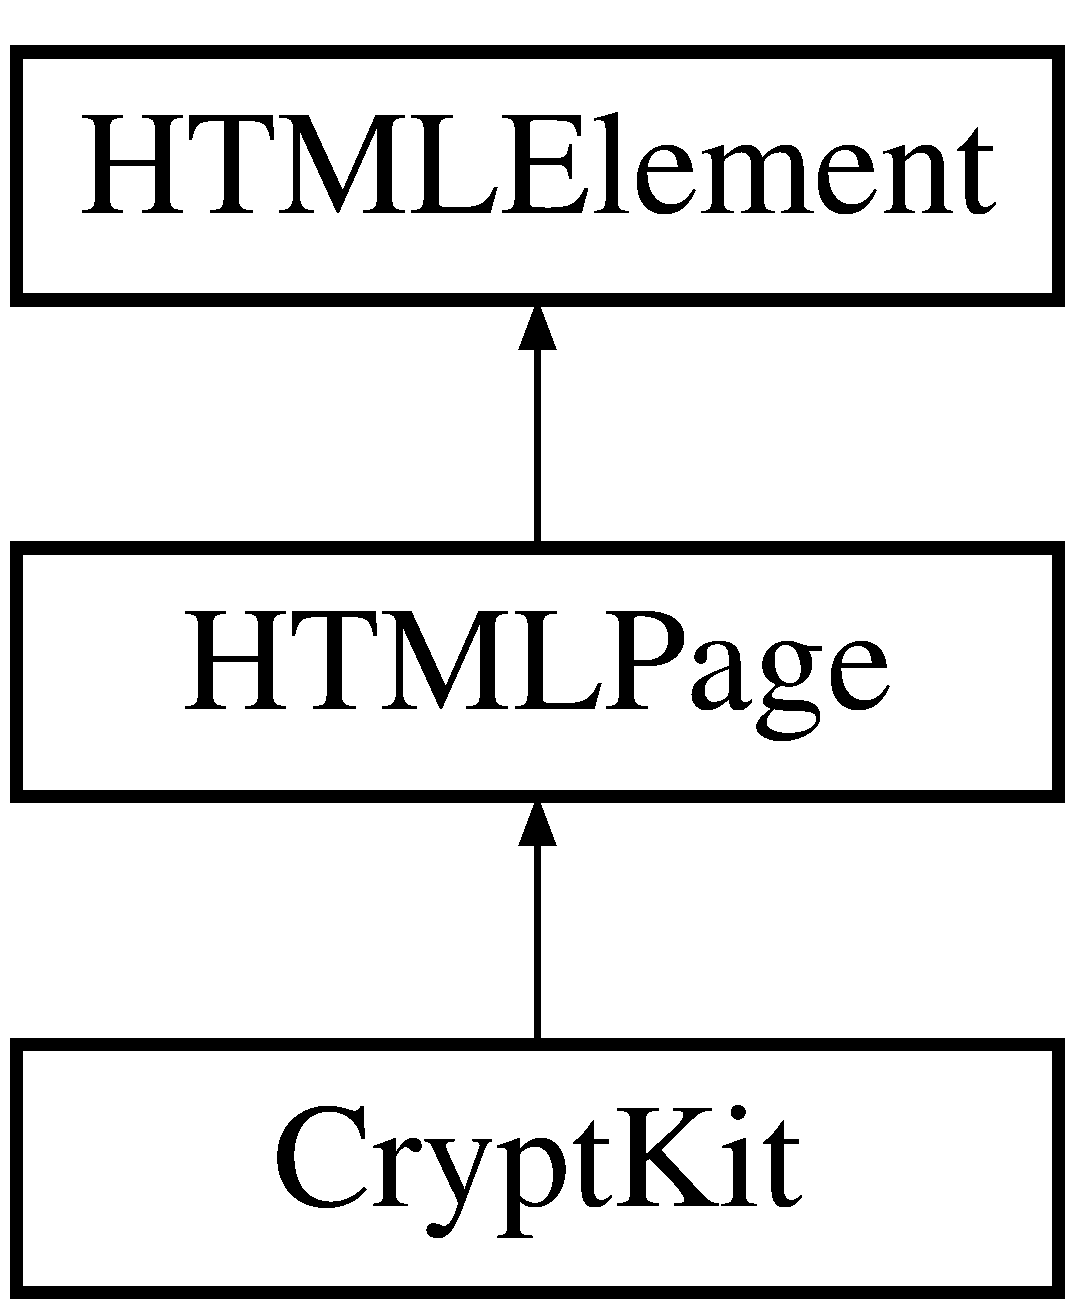
\includegraphics[height=3.000000cm]{class_crypt_kit}
\end{center}
\end{figure}
\subsection*{Public Member Functions}
\begin{DoxyCompactItemize}
\item 
\hyperlink{class_crypt_kit_a63d40b214f91413ccb52cb06be575e50}{encrypt} (\$string, \$key)
\item 
\hyperlink{class_crypt_kit_ae37309b8b5c36f98d3f035415ab5ccee}{decrypt} (\$string, \$key)
\end{DoxyCompactItemize}
\subsection*{Additional Inherited Members}


\subsection{Member Function Documentation}
\hypertarget{class_crypt_kit_ae37309b8b5c36f98d3f035415ab5ccee}{\index{Crypt\-Kit@{Crypt\-Kit}!decrypt@{decrypt}}
\index{decrypt@{decrypt}!CryptKit@{Crypt\-Kit}}
\subsubsection[{decrypt}]{\setlength{\rightskip}{0pt plus 5cm}decrypt (
\begin{DoxyParamCaption}
\item[{}]{\$string, }
\item[{}]{\$key}
\end{DoxyParamCaption}
)}}\label{class_crypt_kit_ae37309b8b5c36f98d3f035415ab5ccee}
\hypertarget{class_crypt_kit_a63d40b214f91413ccb52cb06be575e50}{\index{Crypt\-Kit@{Crypt\-Kit}!encrypt@{encrypt}}
\index{encrypt@{encrypt}!CryptKit@{Crypt\-Kit}}
\subsubsection[{encrypt}]{\setlength{\rightskip}{0pt plus 5cm}encrypt (
\begin{DoxyParamCaption}
\item[{}]{\$string, }
\item[{}]{\$key}
\end{DoxyParamCaption}
)}}\label{class_crypt_kit_a63d40b214f91413ccb52cb06be575e50}


The documentation for this class was generated from the following file\-:\begin{DoxyCompactItemize}
\item 
\hyperlink{pagekit_8php}{pagekit.\-php}\end{DoxyCompactItemize}

\hypertarget{class_d_b_kit}{\section{D\-B\-Kit Class Reference}
\label{class_d_b_kit}\index{D\-B\-Kit@{D\-B\-Kit}}
}
\subsection*{Public Member Functions}
\begin{DoxyCompactItemize}
\item 
\hyperlink{class_d_b_kit_a478255538264e212fe5a3924d69e34a6}{\-\_\-\-\_\-construct} (\$host, \$dbuser, \$dbpassword, \$dbname)
\item 
\hyperlink{class_d_b_kit_a9ac768272a054d6ef7e8436f1144b730}{Connect} ()
\item 
\hyperlink{class_d_b_kit_aec617d8b732c15e5d5be216fee2b9bf5}{Disconnect} ()
\item 
\hyperlink{class_d_b_kit_abe57042ceda608005904adcbf3a03ce1}{Exec\-S\-Q\-L} (\$sql)
\item 
\hyperlink{class_d_b_kit_ab8ad12e8a3f2fed48c7e6974e58f6dcd}{Insert\-Data} (\$table, \$sqlcolumns, \$vars)
\begin{DoxyCompactList}\small\item\em Insert Data into a table. \end{DoxyCompactList}\item 
\hyperlink{class_d_b_kit_a3858bee81ad39a80260c2fc0989ba358}{Fetch\-Data} (\$table, \$sqlcolumns, \$selector)
\begin{DoxyCompactList}\small\item\em Fetch Data into an array. Usage example\-: \$data = \$database-\/$>$Fetch\-Data(\char`\"{}mytable\char`\"{},\char`\"{}$\ast$\char`\"{},\char`\"{}\-O\-R\-D\-E\-R B\-Y id asc\char`\"{});. \end{DoxyCompactList}\item 
\hyperlink{class_d_b_kit_ab2b1c845fbe54b7e22f1ff5901f6c6ce}{Fetch\-Data\-Exec} (\$table, \$sqlcolumns, \$selector)
\item 
\hyperlink{class_d_b_kit_a6de0c2e86c373f77c8833ba52b3f76ce}{Count} ()
\item 
\hyperlink{class_d_b_kit_a6c1483f522f804c83535542ab5938553}{Count\-Table} (\$table)
\item 
\hyperlink{class_d_b_kit_a8daccf2bdab13873d4cdeaf349027bc8}{Mysql} ()
\end{DoxyCompactItemize}
\subsection*{Data Fields}
\begin{DoxyCompactItemize}
\item 
\hyperlink{class_d_b_kit_a112ef069ddc0454086e3d1e6d8d55d07}{\$result}
\end{DoxyCompactItemize}


\subsection{Constructor \& Destructor Documentation}
\hypertarget{class_d_b_kit_a478255538264e212fe5a3924d69e34a6}{\index{D\-B\-Kit@{D\-B\-Kit}!\-\_\-\-\_\-construct@{\-\_\-\-\_\-construct}}
\index{\-\_\-\-\_\-construct@{\-\_\-\-\_\-construct}!DBKit@{D\-B\-Kit}}
\subsubsection[{\-\_\-\-\_\-construct}]{\setlength{\rightskip}{0pt plus 5cm}\-\_\-\-\_\-construct (
\begin{DoxyParamCaption}
\item[{}]{\$host, }
\item[{}]{\$dbuser, }
\item[{}]{\$dbpassword, }
\item[{}]{\$dbname}
\end{DoxyParamCaption}
)}}\label{class_d_b_kit_a478255538264e212fe5a3924d69e34a6}


\subsection{Member Function Documentation}
\hypertarget{class_d_b_kit_a9ac768272a054d6ef7e8436f1144b730}{\index{D\-B\-Kit@{D\-B\-Kit}!Connect@{Connect}}
\index{Connect@{Connect}!DBKit@{D\-B\-Kit}}
\subsubsection[{Connect}]{\setlength{\rightskip}{0pt plus 5cm}Connect (
\begin{DoxyParamCaption}
{}
\end{DoxyParamCaption}
)}}\label{class_d_b_kit_a9ac768272a054d6ef7e8436f1144b730}
\hypertarget{class_d_b_kit_a6de0c2e86c373f77c8833ba52b3f76ce}{\index{D\-B\-Kit@{D\-B\-Kit}!Count@{Count}}
\index{Count@{Count}!DBKit@{D\-B\-Kit}}
\subsubsection[{Count}]{\setlength{\rightskip}{0pt plus 5cm}Count (
\begin{DoxyParamCaption}
{}
\end{DoxyParamCaption}
)}}\label{class_d_b_kit_a6de0c2e86c373f77c8833ba52b3f76ce}
\hypertarget{class_d_b_kit_a6c1483f522f804c83535542ab5938553}{\index{D\-B\-Kit@{D\-B\-Kit}!Count\-Table@{Count\-Table}}
\index{Count\-Table@{Count\-Table}!DBKit@{D\-B\-Kit}}
\subsubsection[{Count\-Table}]{\setlength{\rightskip}{0pt plus 5cm}Count\-Table (
\begin{DoxyParamCaption}
\item[{}]{\$table}
\end{DoxyParamCaption}
)}}\label{class_d_b_kit_a6c1483f522f804c83535542ab5938553}
\hypertarget{class_d_b_kit_aec617d8b732c15e5d5be216fee2b9bf5}{\index{D\-B\-Kit@{D\-B\-Kit}!Disconnect@{Disconnect}}
\index{Disconnect@{Disconnect}!DBKit@{D\-B\-Kit}}
\subsubsection[{Disconnect}]{\setlength{\rightskip}{0pt plus 5cm}Disconnect (
\begin{DoxyParamCaption}
{}
\end{DoxyParamCaption}
)}}\label{class_d_b_kit_aec617d8b732c15e5d5be216fee2b9bf5}
\hypertarget{class_d_b_kit_abe57042ceda608005904adcbf3a03ce1}{\index{D\-B\-Kit@{D\-B\-Kit}!Exec\-S\-Q\-L@{Exec\-S\-Q\-L}}
\index{Exec\-S\-Q\-L@{Exec\-S\-Q\-L}!DBKit@{D\-B\-Kit}}
\subsubsection[{Exec\-S\-Q\-L}]{\setlength{\rightskip}{0pt plus 5cm}Exec\-S\-Q\-L (
\begin{DoxyParamCaption}
\item[{}]{\$sql}
\end{DoxyParamCaption}
)}}\label{class_d_b_kit_abe57042ceda608005904adcbf3a03ce1}
\hypertarget{class_d_b_kit_a3858bee81ad39a80260c2fc0989ba358}{\index{D\-B\-Kit@{D\-B\-Kit}!Fetch\-Data@{Fetch\-Data}}
\index{Fetch\-Data@{Fetch\-Data}!DBKit@{D\-B\-Kit}}
\subsubsection[{Fetch\-Data}]{\setlength{\rightskip}{0pt plus 5cm}Fetch\-Data (
\begin{DoxyParamCaption}
\item[{}]{\$table, }
\item[{}]{\$sqlcolumns, }
\item[{}]{\$selector}
\end{DoxyParamCaption}
)}}\label{class_d_b_kit_a3858bee81ad39a80260c2fc0989ba358}


Fetch Data into an array. Usage example\-: \$data = \$database-\/$>$Fetch\-Data(\char`\"{}mytable\char`\"{},\char`\"{}$\ast$\char`\"{},\char`\"{}\-O\-R\-D\-E\-R B\-Y id asc\char`\"{});. 

foreach (\$data as \$row) \{ \$username = \$row\mbox{[}'username'\mbox{]}; \} \hypertarget{class_d_b_kit_ab2b1c845fbe54b7e22f1ff5901f6c6ce}{\index{D\-B\-Kit@{D\-B\-Kit}!Fetch\-Data\-Exec@{Fetch\-Data\-Exec}}
\index{Fetch\-Data\-Exec@{Fetch\-Data\-Exec}!DBKit@{D\-B\-Kit}}
\subsubsection[{Fetch\-Data\-Exec}]{\setlength{\rightskip}{0pt plus 5cm}Fetch\-Data\-Exec (
\begin{DoxyParamCaption}
\item[{}]{\$table, }
\item[{}]{\$sqlcolumns, }
\item[{}]{\$selector}
\end{DoxyParamCaption}
)}}\label{class_d_b_kit_ab2b1c845fbe54b7e22f1ff5901f6c6ce}
\hypertarget{class_d_b_kit_ab8ad12e8a3f2fed48c7e6974e58f6dcd}{\index{D\-B\-Kit@{D\-B\-Kit}!Insert\-Data@{Insert\-Data}}
\index{Insert\-Data@{Insert\-Data}!DBKit@{D\-B\-Kit}}
\subsubsection[{Insert\-Data}]{\setlength{\rightskip}{0pt plus 5cm}Insert\-Data (
\begin{DoxyParamCaption}
\item[{}]{\$table, }
\item[{}]{\$sqlcolumns, }
\item[{}]{\$vars}
\end{DoxyParamCaption}
)}}\label{class_d_b_kit_ab8ad12e8a3f2fed48c7e6974e58f6dcd}


Insert Data into a table. 

Usage example\-: \$database-\/$>$Insert\-Data(\char`\"{}mytable\char`\"{},\char`\"{}col1,col2,col3\char`\"{},\char`\"{}var1,var2,var3\char`\"{}); \hypertarget{class_d_b_kit_a8daccf2bdab13873d4cdeaf349027bc8}{\index{D\-B\-Kit@{D\-B\-Kit}!Mysql@{Mysql}}
\index{Mysql@{Mysql}!DBKit@{D\-B\-Kit}}
\subsubsection[{Mysql}]{\setlength{\rightskip}{0pt plus 5cm}Mysql (
\begin{DoxyParamCaption}
{}
\end{DoxyParamCaption}
)}}\label{class_d_b_kit_a8daccf2bdab13873d4cdeaf349027bc8}


\subsection{Field Documentation}
\hypertarget{class_d_b_kit_a112ef069ddc0454086e3d1e6d8d55d07}{\index{D\-B\-Kit@{D\-B\-Kit}!\$result@{\$result}}
\index{\$result@{\$result}!DBKit@{D\-B\-Kit}}
\subsubsection[{\$result}]{\setlength{\rightskip}{0pt plus 5cm}\$result}}\label{class_d_b_kit_a112ef069ddc0454086e3d1e6d8d55d07}


The documentation for this class was generated from the following file\-:\begin{DoxyCompactItemize}
\item 
\hyperlink{pagekit_8php}{pagekit.\-php}\end{DoxyCompactItemize}

\hypertarget{class_file_kit}{\section{File\-Kit Class Reference}
\label{class_file_kit}\index{File\-Kit@{File\-Kit}}
}
\subsection*{Public Member Functions}
\begin{DoxyCompactItemize}
\item 
\hyperlink{class_file_kit_a9f764257e50ed47db612375f3f8229b8}{\-\_\-\-\_\-construct} (\$filename, \$mode)
\item 
\hyperlink{class_file_kit_a562791cf1fa35cfd068a27889484e52d}{Set\-Content} (\$content)
\item 
\hyperlink{class_file_kit_a3d385efef707196dfbb556a213c167fd}{Add\-Line} (\$line)
\item 
\hyperlink{class_file_kit_a9258662f7f9ab8c3b67f4fc7b7611105}{Clear} ()
\item 
\hyperlink{class_file_kit_a468f27b26848e99368a29515b562caeb}{Read\-File} ()
\item 
\hyperlink{class_file_kit_ac32b5d24d2961dbeacc6112683fb3c11}{Write\-File} ()
\item 
\hyperlink{class_file_kit_a9f6295ad783c39155d6524205988a110}{Close\-File} ()
\end{DoxyCompactItemize}


\subsection{Constructor \& Destructor Documentation}
\hypertarget{class_file_kit_a9f764257e50ed47db612375f3f8229b8}{\index{File\-Kit@{File\-Kit}!\-\_\-\-\_\-construct@{\-\_\-\-\_\-construct}}
\index{\-\_\-\-\_\-construct@{\-\_\-\-\_\-construct}!FileKit@{File\-Kit}}
\subsubsection[{\-\_\-\-\_\-construct}]{\setlength{\rightskip}{0pt plus 5cm}\-\_\-\-\_\-construct (
\begin{DoxyParamCaption}
\item[{}]{\$filename, }
\item[{}]{\$mode}
\end{DoxyParamCaption}
)}}\label{class_file_kit_a9f764257e50ed47db612375f3f8229b8}


\subsection{Member Function Documentation}
\hypertarget{class_file_kit_a3d385efef707196dfbb556a213c167fd}{\index{File\-Kit@{File\-Kit}!Add\-Line@{Add\-Line}}
\index{Add\-Line@{Add\-Line}!FileKit@{File\-Kit}}
\subsubsection[{Add\-Line}]{\setlength{\rightskip}{0pt plus 5cm}Add\-Line (
\begin{DoxyParamCaption}
\item[{}]{\$line}
\end{DoxyParamCaption}
)}}\label{class_file_kit_a3d385efef707196dfbb556a213c167fd}
\hypertarget{class_file_kit_a9258662f7f9ab8c3b67f4fc7b7611105}{\index{File\-Kit@{File\-Kit}!Clear@{Clear}}
\index{Clear@{Clear}!FileKit@{File\-Kit}}
\subsubsection[{Clear}]{\setlength{\rightskip}{0pt plus 5cm}Clear (
\begin{DoxyParamCaption}
{}
\end{DoxyParamCaption}
)}}\label{class_file_kit_a9258662f7f9ab8c3b67f4fc7b7611105}
\hypertarget{class_file_kit_a9f6295ad783c39155d6524205988a110}{\index{File\-Kit@{File\-Kit}!Close\-File@{Close\-File}}
\index{Close\-File@{Close\-File}!FileKit@{File\-Kit}}
\subsubsection[{Close\-File}]{\setlength{\rightskip}{0pt plus 5cm}Close\-File (
\begin{DoxyParamCaption}
{}
\end{DoxyParamCaption}
)}}\label{class_file_kit_a9f6295ad783c39155d6524205988a110}
\hypertarget{class_file_kit_a468f27b26848e99368a29515b562caeb}{\index{File\-Kit@{File\-Kit}!Read\-File@{Read\-File}}
\index{Read\-File@{Read\-File}!FileKit@{File\-Kit}}
\subsubsection[{Read\-File}]{\setlength{\rightskip}{0pt plus 5cm}Read\-File (
\begin{DoxyParamCaption}
{}
\end{DoxyParamCaption}
)}}\label{class_file_kit_a468f27b26848e99368a29515b562caeb}
\hypertarget{class_file_kit_a562791cf1fa35cfd068a27889484e52d}{\index{File\-Kit@{File\-Kit}!Set\-Content@{Set\-Content}}
\index{Set\-Content@{Set\-Content}!FileKit@{File\-Kit}}
\subsubsection[{Set\-Content}]{\setlength{\rightskip}{0pt plus 5cm}Set\-Content (
\begin{DoxyParamCaption}
\item[{}]{\$content}
\end{DoxyParamCaption}
)}}\label{class_file_kit_a562791cf1fa35cfd068a27889484e52d}
\hypertarget{class_file_kit_ac32b5d24d2961dbeacc6112683fb3c11}{\index{File\-Kit@{File\-Kit}!Write\-File@{Write\-File}}
\index{Write\-File@{Write\-File}!FileKit@{File\-Kit}}
\subsubsection[{Write\-File}]{\setlength{\rightskip}{0pt plus 5cm}Write\-File (
\begin{DoxyParamCaption}
{}
\end{DoxyParamCaption}
)}}\label{class_file_kit_ac32b5d24d2961dbeacc6112683fb3c11}


The documentation for this class was generated from the following file\-:\begin{DoxyCompactItemize}
\item 
\hyperlink{pagekit_8php}{pagekit.\-php}\end{DoxyCompactItemize}

\hypertarget{class_form}{\section{Form Class Reference}
\label{class_form}\index{Form@{Form}}
}
Inheritance diagram for Form\-:\begin{figure}[H]
\begin{center}
\leavevmode
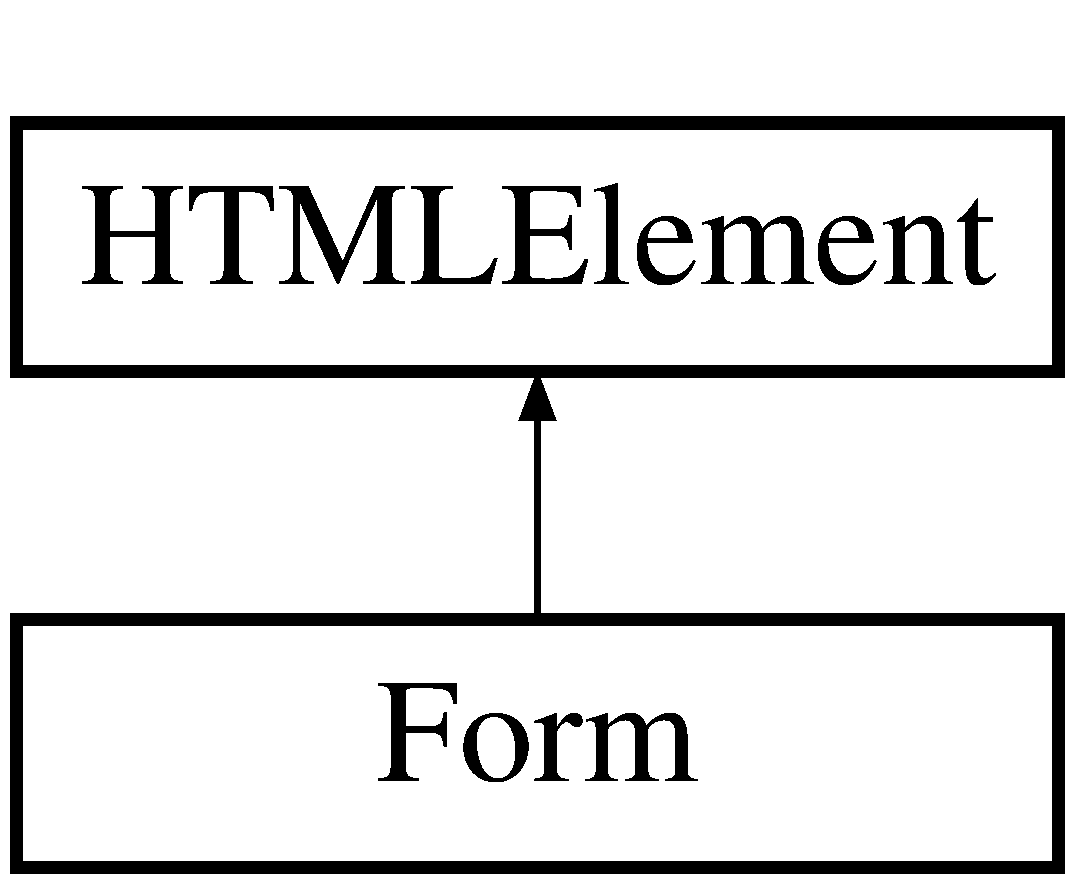
\includegraphics[height=2.000000cm]{class_form}
\end{center}
\end{figure}
\subsection*{Public Member Functions}
\begin{DoxyCompactItemize}
\item 
\hyperlink{class_form_af8e0b4973827723e65906c95202d1f21}{\-\_\-\-\_\-construct} (\$url)
\item 
\hyperlink{class_form_a7deb0d31f66b40e05275d35a0dd7df8a}{Start\-Fieldset} ()
\item 
\hyperlink{class_form_aeddc442ce366a4b306e7a2119e3dfa2a}{End\-Fieldset} ()
\item 
\hyperlink{class_form_abad660ab16e27fe886fa1ab94aa59fc6}{Start\-Group} ()
\item 
\hyperlink{class_form_a93d09060c95897b16ce80c1ff9d63c3f}{End\-Group} ()
\item 
\hyperlink{class_form_a04dcb3227fd89fd80faa6fa703ad0473}{Add\-Label} (\$caption, \$for\-I\-D)
\item 
\hyperlink{class_form_aea553a0a93d55c54a812f411c283cc3c}{Add\-Input} (\$id, \$name, \$placeholder)
\item 
\hyperlink{class_form_a5ea98b5e872229f51417bb35f24a1caf}{Add\-Textarea} (\$id, \$name, \$rows, \$content)
\item 
\hyperlink{class_form_ab01eeca79c10736be036f6f290c543f2}{Add\-Radiobox} (\$id, \$name, \$value, \$checked)
\item 
\hyperlink{class_form_a670614e87d32070235c9ac51252ccb04}{Add\-Checkbox} (\$id, \$name, \$value, \$checked)
\item 
\hyperlink{class_form_aa12881f537f967efd9a4665254dc0a8c}{Add\-Submit} (\$caption)
\end{DoxyCompactItemize}
\subsection*{Additional Inherited Members}


\subsection{Detailed Description}
H\-T\-T\-P \hyperlink{class_form}{Form} Class 

\subsection{Constructor \& Destructor Documentation}
\hypertarget{class_form_af8e0b4973827723e65906c95202d1f21}{\index{Form@{Form}!\-\_\-\-\_\-construct@{\-\_\-\-\_\-construct}}
\index{\-\_\-\-\_\-construct@{\-\_\-\-\_\-construct}!Form@{Form}}
\subsubsection[{\-\_\-\-\_\-construct}]{\setlength{\rightskip}{0pt plus 5cm}\-\_\-\-\_\-construct (
\begin{DoxyParamCaption}
\item[{}]{\$url}
\end{DoxyParamCaption}
)}}\label{class_form_af8e0b4973827723e65906c95202d1f21}


\subsection{Member Function Documentation}
\hypertarget{class_form_a670614e87d32070235c9ac51252ccb04}{\index{Form@{Form}!Add\-Checkbox@{Add\-Checkbox}}
\index{Add\-Checkbox@{Add\-Checkbox}!Form@{Form}}
\subsubsection[{Add\-Checkbox}]{\setlength{\rightskip}{0pt plus 5cm}Add\-Checkbox (
\begin{DoxyParamCaption}
\item[{}]{\$id, }
\item[{}]{\$name, }
\item[{}]{\$value, }
\item[{}]{\$checked}
\end{DoxyParamCaption}
)}}\label{class_form_a670614e87d32070235c9ac51252ccb04}
\hypertarget{class_form_aea553a0a93d55c54a812f411c283cc3c}{\index{Form@{Form}!Add\-Input@{Add\-Input}}
\index{Add\-Input@{Add\-Input}!Form@{Form}}
\subsubsection[{Add\-Input}]{\setlength{\rightskip}{0pt plus 5cm}Add\-Input (
\begin{DoxyParamCaption}
\item[{}]{\$id, }
\item[{}]{\$name, }
\item[{}]{\$placeholder}
\end{DoxyParamCaption}
)}}\label{class_form_aea553a0a93d55c54a812f411c283cc3c}
\hypertarget{class_form_a04dcb3227fd89fd80faa6fa703ad0473}{\index{Form@{Form}!Add\-Label@{Add\-Label}}
\index{Add\-Label@{Add\-Label}!Form@{Form}}
\subsubsection[{Add\-Label}]{\setlength{\rightskip}{0pt plus 5cm}Add\-Label (
\begin{DoxyParamCaption}
\item[{}]{\$caption, }
\item[{}]{\$for\-I\-D}
\end{DoxyParamCaption}
)}}\label{class_form_a04dcb3227fd89fd80faa6fa703ad0473}
\hypertarget{class_form_ab01eeca79c10736be036f6f290c543f2}{\index{Form@{Form}!Add\-Radiobox@{Add\-Radiobox}}
\index{Add\-Radiobox@{Add\-Radiobox}!Form@{Form}}
\subsubsection[{Add\-Radiobox}]{\setlength{\rightskip}{0pt plus 5cm}Add\-Radiobox (
\begin{DoxyParamCaption}
\item[{}]{\$id, }
\item[{}]{\$name, }
\item[{}]{\$value, }
\item[{}]{\$checked}
\end{DoxyParamCaption}
)}}\label{class_form_ab01eeca79c10736be036f6f290c543f2}
\hypertarget{class_form_aa12881f537f967efd9a4665254dc0a8c}{\index{Form@{Form}!Add\-Submit@{Add\-Submit}}
\index{Add\-Submit@{Add\-Submit}!Form@{Form}}
\subsubsection[{Add\-Submit}]{\setlength{\rightskip}{0pt plus 5cm}Add\-Submit (
\begin{DoxyParamCaption}
\item[{}]{\$caption}
\end{DoxyParamCaption}
)}}\label{class_form_aa12881f537f967efd9a4665254dc0a8c}
\hypertarget{class_form_a5ea98b5e872229f51417bb35f24a1caf}{\index{Form@{Form}!Add\-Textarea@{Add\-Textarea}}
\index{Add\-Textarea@{Add\-Textarea}!Form@{Form}}
\subsubsection[{Add\-Textarea}]{\setlength{\rightskip}{0pt plus 5cm}Add\-Textarea (
\begin{DoxyParamCaption}
\item[{}]{\$id, }
\item[{}]{\$name, }
\item[{}]{\$rows, }
\item[{}]{\$content}
\end{DoxyParamCaption}
)}}\label{class_form_a5ea98b5e872229f51417bb35f24a1caf}
\hypertarget{class_form_aeddc442ce366a4b306e7a2119e3dfa2a}{\index{Form@{Form}!End\-Fieldset@{End\-Fieldset}}
\index{End\-Fieldset@{End\-Fieldset}!Form@{Form}}
\subsubsection[{End\-Fieldset}]{\setlength{\rightskip}{0pt plus 5cm}End\-Fieldset (
\begin{DoxyParamCaption}
{}
\end{DoxyParamCaption}
)}}\label{class_form_aeddc442ce366a4b306e7a2119e3dfa2a}
\hypertarget{class_form_a93d09060c95897b16ce80c1ff9d63c3f}{\index{Form@{Form}!End\-Group@{End\-Group}}
\index{End\-Group@{End\-Group}!Form@{Form}}
\subsubsection[{End\-Group}]{\setlength{\rightskip}{0pt plus 5cm}End\-Group (
\begin{DoxyParamCaption}
{}
\end{DoxyParamCaption}
)}}\label{class_form_a93d09060c95897b16ce80c1ff9d63c3f}
\hypertarget{class_form_a7deb0d31f66b40e05275d35a0dd7df8a}{\index{Form@{Form}!Start\-Fieldset@{Start\-Fieldset}}
\index{Start\-Fieldset@{Start\-Fieldset}!Form@{Form}}
\subsubsection[{Start\-Fieldset}]{\setlength{\rightskip}{0pt plus 5cm}Start\-Fieldset (
\begin{DoxyParamCaption}
{}
\end{DoxyParamCaption}
)}}\label{class_form_a7deb0d31f66b40e05275d35a0dd7df8a}
\hypertarget{class_form_abad660ab16e27fe886fa1ab94aa59fc6}{\index{Form@{Form}!Start\-Group@{Start\-Group}}
\index{Start\-Group@{Start\-Group}!Form@{Form}}
\subsubsection[{Start\-Group}]{\setlength{\rightskip}{0pt plus 5cm}Start\-Group (
\begin{DoxyParamCaption}
{}
\end{DoxyParamCaption}
)}}\label{class_form_abad660ab16e27fe886fa1ab94aa59fc6}


The documentation for this class was generated from the following file\-:\begin{DoxyCompactItemize}
\item 
\hyperlink{pagekit_8php}{pagekit.\-php}\end{DoxyCompactItemize}

\hypertarget{class_h_t_m_l_element}{\section{H\-T\-M\-L\-Element Class Reference}
\label{class_h_t_m_l_element}\index{H\-T\-M\-L\-Element@{H\-T\-M\-L\-Element}}
}
Inheritance diagram for H\-T\-M\-L\-Element\-:\begin{figure}[H]
\begin{center}
\leavevmode
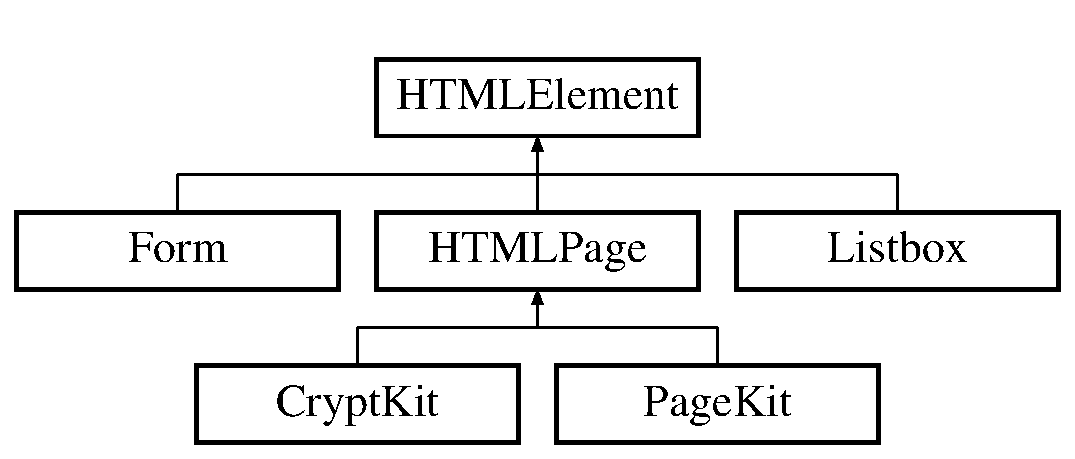
\includegraphics[height=3.000000cm]{class_h_t_m_l_element}
\end{center}
\end{figure}
\subsection*{Public Member Functions}
\begin{DoxyCompactItemize}
\item 
\hyperlink{class_h_t_m_l_element_ac197ac8a1494f06f80566cdb976c84f2}{Init\-H\-T\-M\-L} (\$init)
\item 
\hyperlink{class_h_t_m_l_element_abe647c0d9260043b30261004c312a677}{Finish\-H\-T\-M\-L} (\$finish)
\item 
\hyperlink{class_h_t_m_l_element_a7fd6d1b0467b34de443953e2be12f13a}{Add\-Content} (\$content)
\item 
\hyperlink{class_h_t_m_l_element_ab6b3c0bcc63179b23cc42c901110a16c}{Add\-Menu} ()
\item 
\hyperlink{class_h_t_m_l_element_a29554ae71b8e59155b7d577904748cea}{I\-Frame} (\$width, \$height, \$src, \$border)
\item 
\hyperlink{class_h_t_m_l_element_a989f4d003ff6317129d4eb0785ef32b4}{Text} (\$content)
\item 
\hyperlink{class_h_t_m_l_element_a88a8152792e2d728d1d0f6a1cf0ffb8b}{N\-L} ()
\item 
\hyperlink{class_h_t_m_l_element_a44f142bef7f2fbffa8b2b0c210727787}{L} ()
\item 
\hyperlink{class_h_t_m_l_element_a71e3dc5b5a7a630f66df78a8e1ee2cd4}{Num} (\$number)
\item 
\hyperlink{class_h_t_m_l_element_a96876d2da9cddd39d485bae3d2438c6d}{B} (\$content)
\item 
\hyperlink{class_h_t_m_l_element_a6a372849ec36e5db4047f91f73f3c581}{U} (\$content)
\item 
\hyperlink{class_h_t_m_l_element_a19811fe818d034aab7ec65cb9fc7e0f5}{K} (\$content)
\item 
\hyperlink{class_h_t_m_l_element_a62e160c7f8420244190d71a3775daeea}{D} (\$class, \$content)
\item 
\hyperlink{class_h_t_m_l_element_aeae2417aee112aaca26bbbefe0aa7e10}{D\-S} ()
\item 
\hyperlink{class_h_t_m_l_element_a19f7acb2a4b14e17b749eb10c06b75d9}{D\-E} ()
\item 
\hyperlink{class_h_t_m_l_element_abec61a303902458224a1d7a665093034}{P} (\$content)
\item 
\hyperlink{class_h_t_m_l_element_a84707fade07f58f2de68d5d3d28be365}{Link} (\$url, \$txt, \$target)
\item 
\hyperlink{class_h_t_m_l_element_ac636f824becc1ace9d62b83cf6431f11}{Button} (\$url, \$text, \$size, \$color)
\item 
\hyperlink{class_h_t_m_l_element_a254daefab61356a01c67594c1a94b3b0}{Set\-H\-T\-M\-L} (\$content)
\item 
\hyperlink{class_h_t_m_l_element_ac9f196011988c5ae428ebd5127da8d71}{Get\-Content} ()
\item 
\hyperlink{class_h_t_m_l_element_abc99f9ea27a455eed49d783d5e03c4ad}{Get\-H\-T\-M\-L} ()
\item 
\hyperlink{class_h_t_m_l_element_a9258662f7f9ab8c3b67f4fc7b7611105}{Clear} ()
\item 
\hyperlink{class_h_t_m_l_element_a1a6915de89093bc6383d7c1f18ab81e2}{Render} ()
\end{DoxyCompactItemize}
\subsection*{Protected Attributes}
\begin{DoxyCompactItemize}
\item 
\hyperlink{class_h_t_m_l_element_a6f96e7fc92441776c9d1cd3386663b40}{\$html}
\item 
\hyperlink{class_h_t_m_l_element_a8834b0851b05d161c207a7d2e5dca9bd}{\$init}
\item 
\hyperlink{class_h_t_m_l_element_a63f4f7fe2d310cedeb87d58bd4e45ada}{\$finish}
\end{DoxyCompactItemize}


\subsection{Member Function Documentation}
\hypertarget{class_h_t_m_l_element_a7fd6d1b0467b34de443953e2be12f13a}{\index{H\-T\-M\-L\-Element@{H\-T\-M\-L\-Element}!Add\-Content@{Add\-Content}}
\index{Add\-Content@{Add\-Content}!HTMLElement@{H\-T\-M\-L\-Element}}
\subsubsection[{Add\-Content}]{\setlength{\rightskip}{0pt plus 5cm}Add\-Content (
\begin{DoxyParamCaption}
\item[{}]{\$content}
\end{DoxyParamCaption}
)}}\label{class_h_t_m_l_element_a7fd6d1b0467b34de443953e2be12f13a}
\hypertarget{class_h_t_m_l_element_ab6b3c0bcc63179b23cc42c901110a16c}{\index{H\-T\-M\-L\-Element@{H\-T\-M\-L\-Element}!Add\-Menu@{Add\-Menu}}
\index{Add\-Menu@{Add\-Menu}!HTMLElement@{H\-T\-M\-L\-Element}}
\subsubsection[{Add\-Menu}]{\setlength{\rightskip}{0pt plus 5cm}Add\-Menu (
\begin{DoxyParamCaption}
{}
\end{DoxyParamCaption}
)}}\label{class_h_t_m_l_element_ab6b3c0bcc63179b23cc42c901110a16c}
\hypertarget{class_h_t_m_l_element_a96876d2da9cddd39d485bae3d2438c6d}{\index{H\-T\-M\-L\-Element@{H\-T\-M\-L\-Element}!B@{B}}
\index{B@{B}!HTMLElement@{H\-T\-M\-L\-Element}}
\subsubsection[{B}]{\setlength{\rightskip}{0pt plus 5cm}B (
\begin{DoxyParamCaption}
\item[{}]{\$content}
\end{DoxyParamCaption}
)}}\label{class_h_t_m_l_element_a96876d2da9cddd39d485bae3d2438c6d}
\hypertarget{class_h_t_m_l_element_ac636f824becc1ace9d62b83cf6431f11}{\index{H\-T\-M\-L\-Element@{H\-T\-M\-L\-Element}!Button@{Button}}
\index{Button@{Button}!HTMLElement@{H\-T\-M\-L\-Element}}
\subsubsection[{Button}]{\setlength{\rightskip}{0pt plus 5cm}Button (
\begin{DoxyParamCaption}
\item[{}]{\$url, }
\item[{}]{\$text, }
\item[{}]{\$size, }
\item[{}]{\$color}
\end{DoxyParamCaption}
)}}\label{class_h_t_m_l_element_ac636f824becc1ace9d62b83cf6431f11}
\hypertarget{class_h_t_m_l_element_a9258662f7f9ab8c3b67f4fc7b7611105}{\index{H\-T\-M\-L\-Element@{H\-T\-M\-L\-Element}!Clear@{Clear}}
\index{Clear@{Clear}!HTMLElement@{H\-T\-M\-L\-Element}}
\subsubsection[{Clear}]{\setlength{\rightskip}{0pt plus 5cm}Clear (
\begin{DoxyParamCaption}
{}
\end{DoxyParamCaption}
)}}\label{class_h_t_m_l_element_a9258662f7f9ab8c3b67f4fc7b7611105}
\hypertarget{class_h_t_m_l_element_a62e160c7f8420244190d71a3775daeea}{\index{H\-T\-M\-L\-Element@{H\-T\-M\-L\-Element}!D@{D}}
\index{D@{D}!HTMLElement@{H\-T\-M\-L\-Element}}
\subsubsection[{D}]{\setlength{\rightskip}{0pt plus 5cm}D (
\begin{DoxyParamCaption}
\item[{}]{\$class, }
\item[{}]{\$content}
\end{DoxyParamCaption}
)}}\label{class_h_t_m_l_element_a62e160c7f8420244190d71a3775daeea}
\hypertarget{class_h_t_m_l_element_a19f7acb2a4b14e17b749eb10c06b75d9}{\index{H\-T\-M\-L\-Element@{H\-T\-M\-L\-Element}!D\-E@{D\-E}}
\index{D\-E@{D\-E}!HTMLElement@{H\-T\-M\-L\-Element}}
\subsubsection[{D\-E}]{\setlength{\rightskip}{0pt plus 5cm}D\-E (
\begin{DoxyParamCaption}
{}
\end{DoxyParamCaption}
)}}\label{class_h_t_m_l_element_a19f7acb2a4b14e17b749eb10c06b75d9}
\hypertarget{class_h_t_m_l_element_aeae2417aee112aaca26bbbefe0aa7e10}{\index{H\-T\-M\-L\-Element@{H\-T\-M\-L\-Element}!D\-S@{D\-S}}
\index{D\-S@{D\-S}!HTMLElement@{H\-T\-M\-L\-Element}}
\subsubsection[{D\-S}]{\setlength{\rightskip}{0pt plus 5cm}D\-S (
\begin{DoxyParamCaption}
{}
\end{DoxyParamCaption}
)}}\label{class_h_t_m_l_element_aeae2417aee112aaca26bbbefe0aa7e10}
\hypertarget{class_h_t_m_l_element_abe647c0d9260043b30261004c312a677}{\index{H\-T\-M\-L\-Element@{H\-T\-M\-L\-Element}!Finish\-H\-T\-M\-L@{Finish\-H\-T\-M\-L}}
\index{Finish\-H\-T\-M\-L@{Finish\-H\-T\-M\-L}!HTMLElement@{H\-T\-M\-L\-Element}}
\subsubsection[{Finish\-H\-T\-M\-L}]{\setlength{\rightskip}{0pt plus 5cm}Finish\-H\-T\-M\-L (
\begin{DoxyParamCaption}
\item[{}]{\$finish}
\end{DoxyParamCaption}
)}}\label{class_h_t_m_l_element_abe647c0d9260043b30261004c312a677}
\hypertarget{class_h_t_m_l_element_ac9f196011988c5ae428ebd5127da8d71}{\index{H\-T\-M\-L\-Element@{H\-T\-M\-L\-Element}!Get\-Content@{Get\-Content}}
\index{Get\-Content@{Get\-Content}!HTMLElement@{H\-T\-M\-L\-Element}}
\subsubsection[{Get\-Content}]{\setlength{\rightskip}{0pt plus 5cm}Get\-Content (
\begin{DoxyParamCaption}
{}
\end{DoxyParamCaption}
)}}\label{class_h_t_m_l_element_ac9f196011988c5ae428ebd5127da8d71}
\hypertarget{class_h_t_m_l_element_abc99f9ea27a455eed49d783d5e03c4ad}{\index{H\-T\-M\-L\-Element@{H\-T\-M\-L\-Element}!Get\-H\-T\-M\-L@{Get\-H\-T\-M\-L}}
\index{Get\-H\-T\-M\-L@{Get\-H\-T\-M\-L}!HTMLElement@{H\-T\-M\-L\-Element}}
\subsubsection[{Get\-H\-T\-M\-L}]{\setlength{\rightskip}{0pt plus 5cm}Get\-H\-T\-M\-L (
\begin{DoxyParamCaption}
{}
\end{DoxyParamCaption}
)}}\label{class_h_t_m_l_element_abc99f9ea27a455eed49d783d5e03c4ad}
\hypertarget{class_h_t_m_l_element_a29554ae71b8e59155b7d577904748cea}{\index{H\-T\-M\-L\-Element@{H\-T\-M\-L\-Element}!I\-Frame@{I\-Frame}}
\index{I\-Frame@{I\-Frame}!HTMLElement@{H\-T\-M\-L\-Element}}
\subsubsection[{I\-Frame}]{\setlength{\rightskip}{0pt plus 5cm}I\-Frame (
\begin{DoxyParamCaption}
\item[{}]{\$width, }
\item[{}]{\$height, }
\item[{}]{\$src, }
\item[{}]{\$border}
\end{DoxyParamCaption}
)}}\label{class_h_t_m_l_element_a29554ae71b8e59155b7d577904748cea}
\hypertarget{class_h_t_m_l_element_ac197ac8a1494f06f80566cdb976c84f2}{\index{H\-T\-M\-L\-Element@{H\-T\-M\-L\-Element}!Init\-H\-T\-M\-L@{Init\-H\-T\-M\-L}}
\index{Init\-H\-T\-M\-L@{Init\-H\-T\-M\-L}!HTMLElement@{H\-T\-M\-L\-Element}}
\subsubsection[{Init\-H\-T\-M\-L}]{\setlength{\rightskip}{0pt plus 5cm}Init\-H\-T\-M\-L (
\begin{DoxyParamCaption}
\item[{}]{\$init}
\end{DoxyParamCaption}
)}}\label{class_h_t_m_l_element_ac197ac8a1494f06f80566cdb976c84f2}
\hypertarget{class_h_t_m_l_element_a19811fe818d034aab7ec65cb9fc7e0f5}{\index{H\-T\-M\-L\-Element@{H\-T\-M\-L\-Element}!K@{K}}
\index{K@{K}!HTMLElement@{H\-T\-M\-L\-Element}}
\subsubsection[{K}]{\setlength{\rightskip}{0pt plus 5cm}K (
\begin{DoxyParamCaption}
\item[{}]{\$content}
\end{DoxyParamCaption}
)}}\label{class_h_t_m_l_element_a19811fe818d034aab7ec65cb9fc7e0f5}
\hypertarget{class_h_t_m_l_element_a44f142bef7f2fbffa8b2b0c210727787}{\index{H\-T\-M\-L\-Element@{H\-T\-M\-L\-Element}!L@{L}}
\index{L@{L}!HTMLElement@{H\-T\-M\-L\-Element}}
\subsubsection[{L}]{\setlength{\rightskip}{0pt plus 5cm}L (
\begin{DoxyParamCaption}
{}
\end{DoxyParamCaption}
)}}\label{class_h_t_m_l_element_a44f142bef7f2fbffa8b2b0c210727787}
\hypertarget{class_h_t_m_l_element_a84707fade07f58f2de68d5d3d28be365}{\index{H\-T\-M\-L\-Element@{H\-T\-M\-L\-Element}!Link@{Link}}
\index{Link@{Link}!HTMLElement@{H\-T\-M\-L\-Element}}
\subsubsection[{Link}]{\setlength{\rightskip}{0pt plus 5cm}Link (
\begin{DoxyParamCaption}
\item[{}]{\$url, }
\item[{}]{\$txt, }
\item[{}]{\$target}
\end{DoxyParamCaption}
)}}\label{class_h_t_m_l_element_a84707fade07f58f2de68d5d3d28be365}
\hypertarget{class_h_t_m_l_element_a88a8152792e2d728d1d0f6a1cf0ffb8b}{\index{H\-T\-M\-L\-Element@{H\-T\-M\-L\-Element}!N\-L@{N\-L}}
\index{N\-L@{N\-L}!HTMLElement@{H\-T\-M\-L\-Element}}
\subsubsection[{N\-L}]{\setlength{\rightskip}{0pt plus 5cm}N\-L (
\begin{DoxyParamCaption}
{}
\end{DoxyParamCaption}
)}}\label{class_h_t_m_l_element_a88a8152792e2d728d1d0f6a1cf0ffb8b}
\hypertarget{class_h_t_m_l_element_a71e3dc5b5a7a630f66df78a8e1ee2cd4}{\index{H\-T\-M\-L\-Element@{H\-T\-M\-L\-Element}!Num@{Num}}
\index{Num@{Num}!HTMLElement@{H\-T\-M\-L\-Element}}
\subsubsection[{Num}]{\setlength{\rightskip}{0pt plus 5cm}Num (
\begin{DoxyParamCaption}
\item[{}]{\$number}
\end{DoxyParamCaption}
)}}\label{class_h_t_m_l_element_a71e3dc5b5a7a630f66df78a8e1ee2cd4}
\hypertarget{class_h_t_m_l_element_abec61a303902458224a1d7a665093034}{\index{H\-T\-M\-L\-Element@{H\-T\-M\-L\-Element}!P@{P}}
\index{P@{P}!HTMLElement@{H\-T\-M\-L\-Element}}
\subsubsection[{P}]{\setlength{\rightskip}{0pt plus 5cm}P (
\begin{DoxyParamCaption}
\item[{}]{\$content}
\end{DoxyParamCaption}
)}}\label{class_h_t_m_l_element_abec61a303902458224a1d7a665093034}
\hypertarget{class_h_t_m_l_element_a1a6915de89093bc6383d7c1f18ab81e2}{\index{H\-T\-M\-L\-Element@{H\-T\-M\-L\-Element}!Render@{Render}}
\index{Render@{Render}!HTMLElement@{H\-T\-M\-L\-Element}}
\subsubsection[{Render}]{\setlength{\rightskip}{0pt plus 5cm}Render (
\begin{DoxyParamCaption}
{}
\end{DoxyParamCaption}
)}}\label{class_h_t_m_l_element_a1a6915de89093bc6383d7c1f18ab81e2}
\hypertarget{class_h_t_m_l_element_a254daefab61356a01c67594c1a94b3b0}{\index{H\-T\-M\-L\-Element@{H\-T\-M\-L\-Element}!Set\-H\-T\-M\-L@{Set\-H\-T\-M\-L}}
\index{Set\-H\-T\-M\-L@{Set\-H\-T\-M\-L}!HTMLElement@{H\-T\-M\-L\-Element}}
\subsubsection[{Set\-H\-T\-M\-L}]{\setlength{\rightskip}{0pt plus 5cm}Set\-H\-T\-M\-L (
\begin{DoxyParamCaption}
\item[{}]{\$content}
\end{DoxyParamCaption}
)}}\label{class_h_t_m_l_element_a254daefab61356a01c67594c1a94b3b0}
\hypertarget{class_h_t_m_l_element_a989f4d003ff6317129d4eb0785ef32b4}{\index{H\-T\-M\-L\-Element@{H\-T\-M\-L\-Element}!Text@{Text}}
\index{Text@{Text}!HTMLElement@{H\-T\-M\-L\-Element}}
\subsubsection[{Text}]{\setlength{\rightskip}{0pt plus 5cm}Text (
\begin{DoxyParamCaption}
\item[{}]{\$content}
\end{DoxyParamCaption}
)}}\label{class_h_t_m_l_element_a989f4d003ff6317129d4eb0785ef32b4}
\hypertarget{class_h_t_m_l_element_a6a372849ec36e5db4047f91f73f3c581}{\index{H\-T\-M\-L\-Element@{H\-T\-M\-L\-Element}!U@{U}}
\index{U@{U}!HTMLElement@{H\-T\-M\-L\-Element}}
\subsubsection[{U}]{\setlength{\rightskip}{0pt plus 5cm}U (
\begin{DoxyParamCaption}
\item[{}]{\$content}
\end{DoxyParamCaption}
)}}\label{class_h_t_m_l_element_a6a372849ec36e5db4047f91f73f3c581}


\subsection{Field Documentation}
\hypertarget{class_h_t_m_l_element_a63f4f7fe2d310cedeb87d58bd4e45ada}{\index{H\-T\-M\-L\-Element@{H\-T\-M\-L\-Element}!\$finish@{\$finish}}
\index{\$finish@{\$finish}!HTMLElement@{H\-T\-M\-L\-Element}}
\subsubsection[{\$finish}]{\setlength{\rightskip}{0pt plus 5cm}\$finish\hspace{0.3cm}{\ttfamily [protected]}}}\label{class_h_t_m_l_element_a63f4f7fe2d310cedeb87d58bd4e45ada}
\hypertarget{class_h_t_m_l_element_a6f96e7fc92441776c9d1cd3386663b40}{\index{H\-T\-M\-L\-Element@{H\-T\-M\-L\-Element}!\$html@{\$html}}
\index{\$html@{\$html}!HTMLElement@{H\-T\-M\-L\-Element}}
\subsubsection[{\$html}]{\setlength{\rightskip}{0pt plus 5cm}\$html\hspace{0.3cm}{\ttfamily [protected]}}}\label{class_h_t_m_l_element_a6f96e7fc92441776c9d1cd3386663b40}
\hypertarget{class_h_t_m_l_element_a8834b0851b05d161c207a7d2e5dca9bd}{\index{H\-T\-M\-L\-Element@{H\-T\-M\-L\-Element}!\$init@{\$init}}
\index{\$init@{\$init}!HTMLElement@{H\-T\-M\-L\-Element}}
\subsubsection[{\$init}]{\setlength{\rightskip}{0pt plus 5cm}\$init\hspace{0.3cm}{\ttfamily [protected]}}}\label{class_h_t_m_l_element_a8834b0851b05d161c207a7d2e5dca9bd}


The documentation for this class was generated from the following file\-:\begin{DoxyCompactItemize}
\item 
\hyperlink{pagekit_8php}{pagekit.\-php}\end{DoxyCompactItemize}

\hypertarget{class_h_t_m_l_page}{\section{H\-T\-M\-L\-Page Class Reference}
\label{class_h_t_m_l_page}\index{H\-T\-M\-L\-Page@{H\-T\-M\-L\-Page}}
}
Inheritance diagram for H\-T\-M\-L\-Page\-:\begin{figure}[H]
\begin{center}
\leavevmode
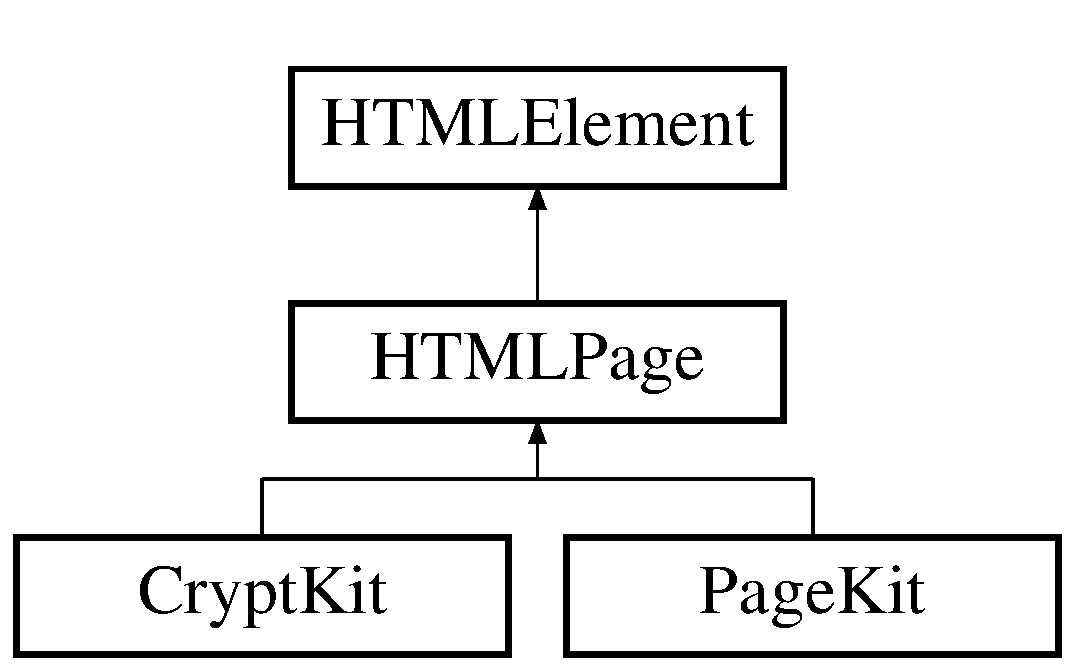
\includegraphics[height=3.000000cm]{class_h_t_m_l_page}
\end{center}
\end{figure}
\subsection*{Public Member Functions}
\begin{DoxyCompactItemize}
\item 
\hyperlink{class_h_t_m_l_page_a6220f56b893af1eeeaa7bb84f6ca13b2}{\-\_\-\-\_\-construct} (\$title)
\item 
\hyperlink{class_h_t_m_l_page_a6a54104bbbaeee3dffbc269b526c70d4}{Add} (\$content)
\item 
\hyperlink{class_h_t_m_l_page_a728d47dc8dffe39b76d0feb6491b437c}{Add\-Header} (\$content)
\item 
\hyperlink{class_h_t_m_l_page_aec006b57e0f96d8b799f0f7ea22871f1}{Play\-Sound} (\$soundurl)
\item 
\hyperlink{class_h_t_m_l_page_a83649c48e61c09d8e80d72163b50d638}{Clear\-Page} ()
\item 
\hyperlink{class_h_t_m_l_page_a1a6915de89093bc6383d7c1f18ab81e2}{Render} ()
\item 
\hyperlink{class_h_t_m_l_page_a205a4450570ca0868c4334c334859be9}{Save\-File} (\$filename)
\end{DoxyCompactItemize}
\subsection*{Protected Attributes}
\begin{DoxyCompactItemize}
\item 
\hyperlink{class_h_t_m_l_page_ada57e7bb7c152edad18fe2f166188691}{\$title}
\item 
\hyperlink{class_h_t_m_l_page_a4f44601f2b9dc8a1644bce53c94ce622}{\$header}
\item 
\hyperlink{class_h_t_m_l_page_a271c9f1463d598b29e28b6642d175365}{\$scripts}
\item 
\hyperlink{class_h_t_m_l_page_a6f96e7fc92441776c9d1cd3386663b40}{\$html}
\end{DoxyCompactItemize}


\subsection{Constructor \& Destructor Documentation}
\hypertarget{class_h_t_m_l_page_a6220f56b893af1eeeaa7bb84f6ca13b2}{\index{H\-T\-M\-L\-Page@{H\-T\-M\-L\-Page}!\-\_\-\-\_\-construct@{\-\_\-\-\_\-construct}}
\index{\-\_\-\-\_\-construct@{\-\_\-\-\_\-construct}!HTMLPage@{H\-T\-M\-L\-Page}}
\subsubsection[{\-\_\-\-\_\-construct}]{\setlength{\rightskip}{0pt plus 5cm}\-\_\-\-\_\-construct (
\begin{DoxyParamCaption}
\item[{}]{\$title}
\end{DoxyParamCaption}
)}}\label{class_h_t_m_l_page_a6220f56b893af1eeeaa7bb84f6ca13b2}


\subsection{Member Function Documentation}
\hypertarget{class_h_t_m_l_page_a6a54104bbbaeee3dffbc269b526c70d4}{\index{H\-T\-M\-L\-Page@{H\-T\-M\-L\-Page}!Add@{Add}}
\index{Add@{Add}!HTMLPage@{H\-T\-M\-L\-Page}}
\subsubsection[{Add}]{\setlength{\rightskip}{0pt plus 5cm}Add (
\begin{DoxyParamCaption}
\item[{}]{\$content}
\end{DoxyParamCaption}
)}}\label{class_h_t_m_l_page_a6a54104bbbaeee3dffbc269b526c70d4}
\hypertarget{class_h_t_m_l_page_a728d47dc8dffe39b76d0feb6491b437c}{\index{H\-T\-M\-L\-Page@{H\-T\-M\-L\-Page}!Add\-Header@{Add\-Header}}
\index{Add\-Header@{Add\-Header}!HTMLPage@{H\-T\-M\-L\-Page}}
\subsubsection[{Add\-Header}]{\setlength{\rightskip}{0pt plus 5cm}Add\-Header (
\begin{DoxyParamCaption}
\item[{}]{\$content}
\end{DoxyParamCaption}
)}}\label{class_h_t_m_l_page_a728d47dc8dffe39b76d0feb6491b437c}
\hypertarget{class_h_t_m_l_page_a83649c48e61c09d8e80d72163b50d638}{\index{H\-T\-M\-L\-Page@{H\-T\-M\-L\-Page}!Clear\-Page@{Clear\-Page}}
\index{Clear\-Page@{Clear\-Page}!HTMLPage@{H\-T\-M\-L\-Page}}
\subsubsection[{Clear\-Page}]{\setlength{\rightskip}{0pt plus 5cm}Clear\-Page (
\begin{DoxyParamCaption}
{}
\end{DoxyParamCaption}
)}}\label{class_h_t_m_l_page_a83649c48e61c09d8e80d72163b50d638}
\hypertarget{class_h_t_m_l_page_aec006b57e0f96d8b799f0f7ea22871f1}{\index{H\-T\-M\-L\-Page@{H\-T\-M\-L\-Page}!Play\-Sound@{Play\-Sound}}
\index{Play\-Sound@{Play\-Sound}!HTMLPage@{H\-T\-M\-L\-Page}}
\subsubsection[{Play\-Sound}]{\setlength{\rightskip}{0pt plus 5cm}Play\-Sound (
\begin{DoxyParamCaption}
\item[{}]{\$soundurl}
\end{DoxyParamCaption}
)}}\label{class_h_t_m_l_page_aec006b57e0f96d8b799f0f7ea22871f1}
\hypertarget{class_h_t_m_l_page_a1a6915de89093bc6383d7c1f18ab81e2}{\index{H\-T\-M\-L\-Page@{H\-T\-M\-L\-Page}!Render@{Render}}
\index{Render@{Render}!HTMLPage@{H\-T\-M\-L\-Page}}
\subsubsection[{Render}]{\setlength{\rightskip}{0pt plus 5cm}Render (
\begin{DoxyParamCaption}
{}
\end{DoxyParamCaption}
)}}\label{class_h_t_m_l_page_a1a6915de89093bc6383d7c1f18ab81e2}
\hypertarget{class_h_t_m_l_page_a205a4450570ca0868c4334c334859be9}{\index{H\-T\-M\-L\-Page@{H\-T\-M\-L\-Page}!Save\-File@{Save\-File}}
\index{Save\-File@{Save\-File}!HTMLPage@{H\-T\-M\-L\-Page}}
\subsubsection[{Save\-File}]{\setlength{\rightskip}{0pt plus 5cm}Save\-File (
\begin{DoxyParamCaption}
\item[{}]{\$filename}
\end{DoxyParamCaption}
)}}\label{class_h_t_m_l_page_a205a4450570ca0868c4334c334859be9}


\subsection{Field Documentation}
\hypertarget{class_h_t_m_l_page_a4f44601f2b9dc8a1644bce53c94ce622}{\index{H\-T\-M\-L\-Page@{H\-T\-M\-L\-Page}!\$header@{\$header}}
\index{\$header@{\$header}!HTMLPage@{H\-T\-M\-L\-Page}}
\subsubsection[{\$header}]{\setlength{\rightskip}{0pt plus 5cm}\$header\hspace{0.3cm}{\ttfamily [protected]}}}\label{class_h_t_m_l_page_a4f44601f2b9dc8a1644bce53c94ce622}
\hypertarget{class_h_t_m_l_page_a6f96e7fc92441776c9d1cd3386663b40}{\index{H\-T\-M\-L\-Page@{H\-T\-M\-L\-Page}!\$html@{\$html}}
\index{\$html@{\$html}!HTMLPage@{H\-T\-M\-L\-Page}}
\subsubsection[{\$html}]{\setlength{\rightskip}{0pt plus 5cm}\$html\hspace{0.3cm}{\ttfamily [protected]}}}\label{class_h_t_m_l_page_a6f96e7fc92441776c9d1cd3386663b40}
\hypertarget{class_h_t_m_l_page_a271c9f1463d598b29e28b6642d175365}{\index{H\-T\-M\-L\-Page@{H\-T\-M\-L\-Page}!\$scripts@{\$scripts}}
\index{\$scripts@{\$scripts}!HTMLPage@{H\-T\-M\-L\-Page}}
\subsubsection[{\$scripts}]{\setlength{\rightskip}{0pt plus 5cm}\$scripts\hspace{0.3cm}{\ttfamily [protected]}}}\label{class_h_t_m_l_page_a271c9f1463d598b29e28b6642d175365}
\hypertarget{class_h_t_m_l_page_ada57e7bb7c152edad18fe2f166188691}{\index{H\-T\-M\-L\-Page@{H\-T\-M\-L\-Page}!\$title@{\$title}}
\index{\$title@{\$title}!HTMLPage@{H\-T\-M\-L\-Page}}
\subsubsection[{\$title}]{\setlength{\rightskip}{0pt plus 5cm}\$title\hspace{0.3cm}{\ttfamily [protected]}}}\label{class_h_t_m_l_page_ada57e7bb7c152edad18fe2f166188691}


The documentation for this class was generated from the following file\-:\begin{DoxyCompactItemize}
\item 
\hyperlink{pagekit_8php}{pagekit.\-php}\end{DoxyCompactItemize}

\hypertarget{class_kit_settings}{\section{Kit\-Settings Class Reference}
\label{class_kit_settings}\index{Kit\-Settings@{Kit\-Settings}}
}
\subsection*{Public Member Functions}
\begin{DoxyCompactItemize}
\item 
\hyperlink{class_kit_settings_adb5b1e3446815a0696917e72f2e20e05}{\-\_\-\-\_\-construct} (\$host, \$dbname, \$dbuser, \$dbpassword)
\end{DoxyCompactItemize}
\subsection*{Data Fields}
\begin{DoxyCompactItemize}
\item 
\hyperlink{class_kit_settings_a711797613cb863ca0756df789c396bf2}{\$host}
\item 
\hyperlink{class_kit_settings_ac5111a571fffa2499732833bb7f0d8c1}{\$dbname}
\item 
\hyperlink{class_kit_settings_a8d5ac1c3396a540f025f9bbe56a5b568}{\$dbuser}
\item 
\hyperlink{class_kit_settings_a0d42c2db361e096182a30d694e0cd6e4}{\$dbpassword}
\end{DoxyCompactItemize}


\subsection{Detailed Description}
\hyperlink{class_page_kit}{Page\-Kit} Settings are stored here 

\subsection{Constructor \& Destructor Documentation}
\hypertarget{class_kit_settings_adb5b1e3446815a0696917e72f2e20e05}{\index{Kit\-Settings@{Kit\-Settings}!\-\_\-\-\_\-construct@{\-\_\-\-\_\-construct}}
\index{\-\_\-\-\_\-construct@{\-\_\-\-\_\-construct}!KitSettings@{Kit\-Settings}}
\subsubsection[{\-\_\-\-\_\-construct}]{\setlength{\rightskip}{0pt plus 5cm}\-\_\-\-\_\-construct (
\begin{DoxyParamCaption}
\item[{}]{\$host, }
\item[{}]{\$dbname, }
\item[{}]{\$dbuser, }
\item[{}]{\$dbpassword}
\end{DoxyParamCaption}
)}}\label{class_kit_settings_adb5b1e3446815a0696917e72f2e20e05}
Initialises the Kit automatically 

\subsection{Field Documentation}
\hypertarget{class_kit_settings_ac5111a571fffa2499732833bb7f0d8c1}{\index{Kit\-Settings@{Kit\-Settings}!\$dbname@{\$dbname}}
\index{\$dbname@{\$dbname}!KitSettings@{Kit\-Settings}}
\subsubsection[{\$dbname}]{\setlength{\rightskip}{0pt plus 5cm}\$dbname}}\label{class_kit_settings_ac5111a571fffa2499732833bb7f0d8c1}
\hypertarget{class_kit_settings_a0d42c2db361e096182a30d694e0cd6e4}{\index{Kit\-Settings@{Kit\-Settings}!\$dbpassword@{\$dbpassword}}
\index{\$dbpassword@{\$dbpassword}!KitSettings@{Kit\-Settings}}
\subsubsection[{\$dbpassword}]{\setlength{\rightskip}{0pt plus 5cm}\$dbpassword}}\label{class_kit_settings_a0d42c2db361e096182a30d694e0cd6e4}
\hypertarget{class_kit_settings_a8d5ac1c3396a540f025f9bbe56a5b568}{\index{Kit\-Settings@{Kit\-Settings}!\$dbuser@{\$dbuser}}
\index{\$dbuser@{\$dbuser}!KitSettings@{Kit\-Settings}}
\subsubsection[{\$dbuser}]{\setlength{\rightskip}{0pt plus 5cm}\$dbuser}}\label{class_kit_settings_a8d5ac1c3396a540f025f9bbe56a5b568}
\hypertarget{class_kit_settings_a711797613cb863ca0756df789c396bf2}{\index{Kit\-Settings@{Kit\-Settings}!\$host@{\$host}}
\index{\$host@{\$host}!KitSettings@{Kit\-Settings}}
\subsubsection[{\$host}]{\setlength{\rightskip}{0pt plus 5cm}\$host}}\label{class_kit_settings_a711797613cb863ca0756df789c396bf2}


The documentation for this class was generated from the following file\-:\begin{DoxyCompactItemize}
\item 
\hyperlink{pagekit_8php}{pagekit.\-php}\end{DoxyCompactItemize}

\hypertarget{class_listbox}{\section{Listbox Class Reference}
\label{class_listbox}\index{Listbox@{Listbox}}
}
Inheritance diagram for Listbox\-:\begin{figure}[H]
\begin{center}
\leavevmode
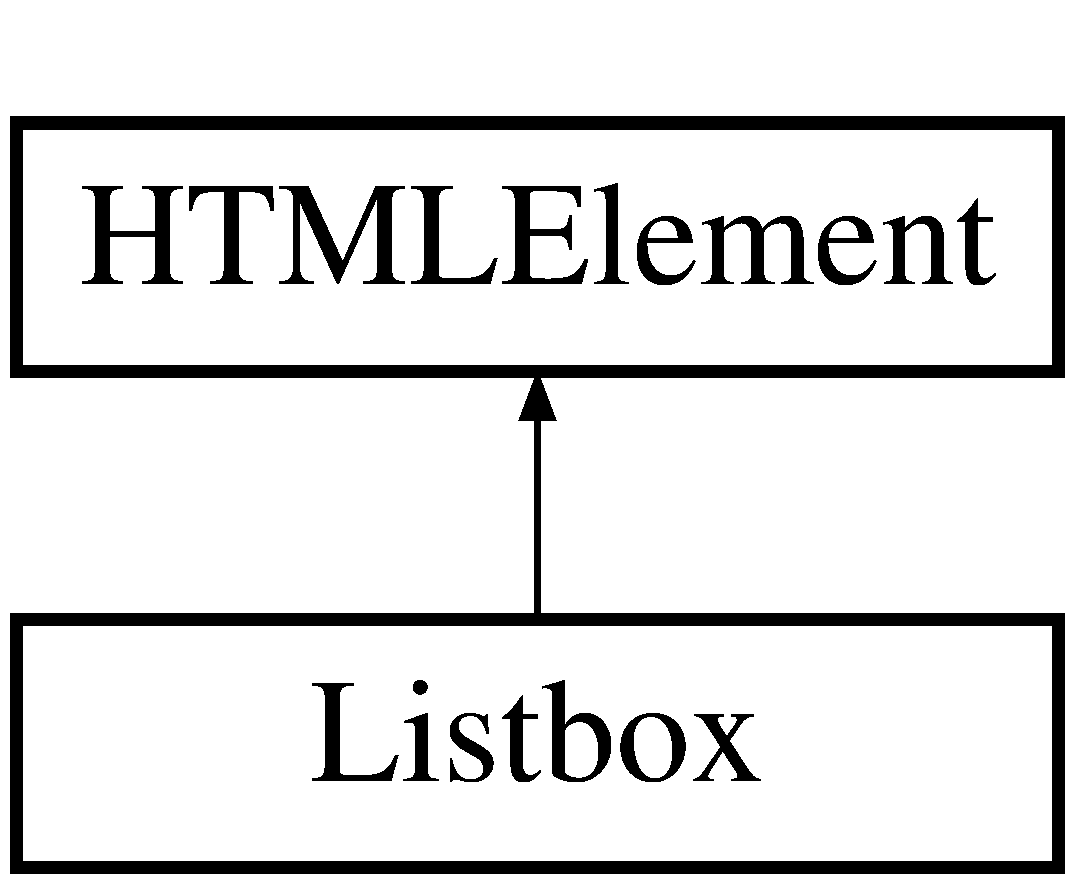
\includegraphics[height=2.000000cm]{class_listbox}
\end{center}
\end{figure}
\subsection*{Public Member Functions}
\begin{DoxyCompactItemize}
\item 
\hyperlink{class_listbox_a8b286130867713c4f960c815e1047f98}{\-\_\-\-\_\-construct} (\$id, \$name, \$size, \$multiple)
\item 
\hyperlink{class_listbox_a51500c8d46491f007a83e20a90da222d}{Start\-Group} (\$title)
\item 
\hyperlink{class_listbox_a93d09060c95897b16ce80c1ff9d63c3f}{End\-Group} ()
\item 
\hyperlink{class_listbox_a97e06b451dbb8a1ced1297b781926946}{Add\-Option} (\$option, \$value, \$selected)
\end{DoxyCompactItemize}
\subsection*{Additional Inherited Members}


\subsection{Constructor \& Destructor Documentation}
\hypertarget{class_listbox_a8b286130867713c4f960c815e1047f98}{\index{Listbox@{Listbox}!\-\_\-\-\_\-construct@{\-\_\-\-\_\-construct}}
\index{\-\_\-\-\_\-construct@{\-\_\-\-\_\-construct}!Listbox@{Listbox}}
\subsubsection[{\-\_\-\-\_\-construct}]{\setlength{\rightskip}{0pt plus 5cm}\-\_\-\-\_\-construct (
\begin{DoxyParamCaption}
\item[{}]{\$id, }
\item[{}]{\$name, }
\item[{}]{\$size, }
\item[{}]{\$multiple}
\end{DoxyParamCaption}
)}}\label{class_listbox_a8b286130867713c4f960c815e1047f98}


\subsection{Member Function Documentation}
\hypertarget{class_listbox_a97e06b451dbb8a1ced1297b781926946}{\index{Listbox@{Listbox}!Add\-Option@{Add\-Option}}
\index{Add\-Option@{Add\-Option}!Listbox@{Listbox}}
\subsubsection[{Add\-Option}]{\setlength{\rightskip}{0pt plus 5cm}Add\-Option (
\begin{DoxyParamCaption}
\item[{}]{\$option, }
\item[{}]{\$value, }
\item[{}]{\$selected}
\end{DoxyParamCaption}
)}}\label{class_listbox_a97e06b451dbb8a1ced1297b781926946}
\hypertarget{class_listbox_a93d09060c95897b16ce80c1ff9d63c3f}{\index{Listbox@{Listbox}!End\-Group@{End\-Group}}
\index{End\-Group@{End\-Group}!Listbox@{Listbox}}
\subsubsection[{End\-Group}]{\setlength{\rightskip}{0pt plus 5cm}End\-Group (
\begin{DoxyParamCaption}
{}
\end{DoxyParamCaption}
)}}\label{class_listbox_a93d09060c95897b16ce80c1ff9d63c3f}
\hypertarget{class_listbox_a51500c8d46491f007a83e20a90da222d}{\index{Listbox@{Listbox}!Start\-Group@{Start\-Group}}
\index{Start\-Group@{Start\-Group}!Listbox@{Listbox}}
\subsubsection[{Start\-Group}]{\setlength{\rightskip}{0pt plus 5cm}Start\-Group (
\begin{DoxyParamCaption}
\item[{}]{\$title}
\end{DoxyParamCaption}
)}}\label{class_listbox_a51500c8d46491f007a83e20a90da222d}


The documentation for this class was generated from the following file\-:\begin{DoxyCompactItemize}
\item 
\hyperlink{pagekit_8php}{pagekit.\-php}\end{DoxyCompactItemize}

\hypertarget{class_page_kit}{\section{Page\-Kit Class Reference}
\label{class_page_kit}\index{Page\-Kit@{Page\-Kit}}
}
Inheritance diagram for Page\-Kit\-:\begin{figure}[H]
\begin{center}
\leavevmode
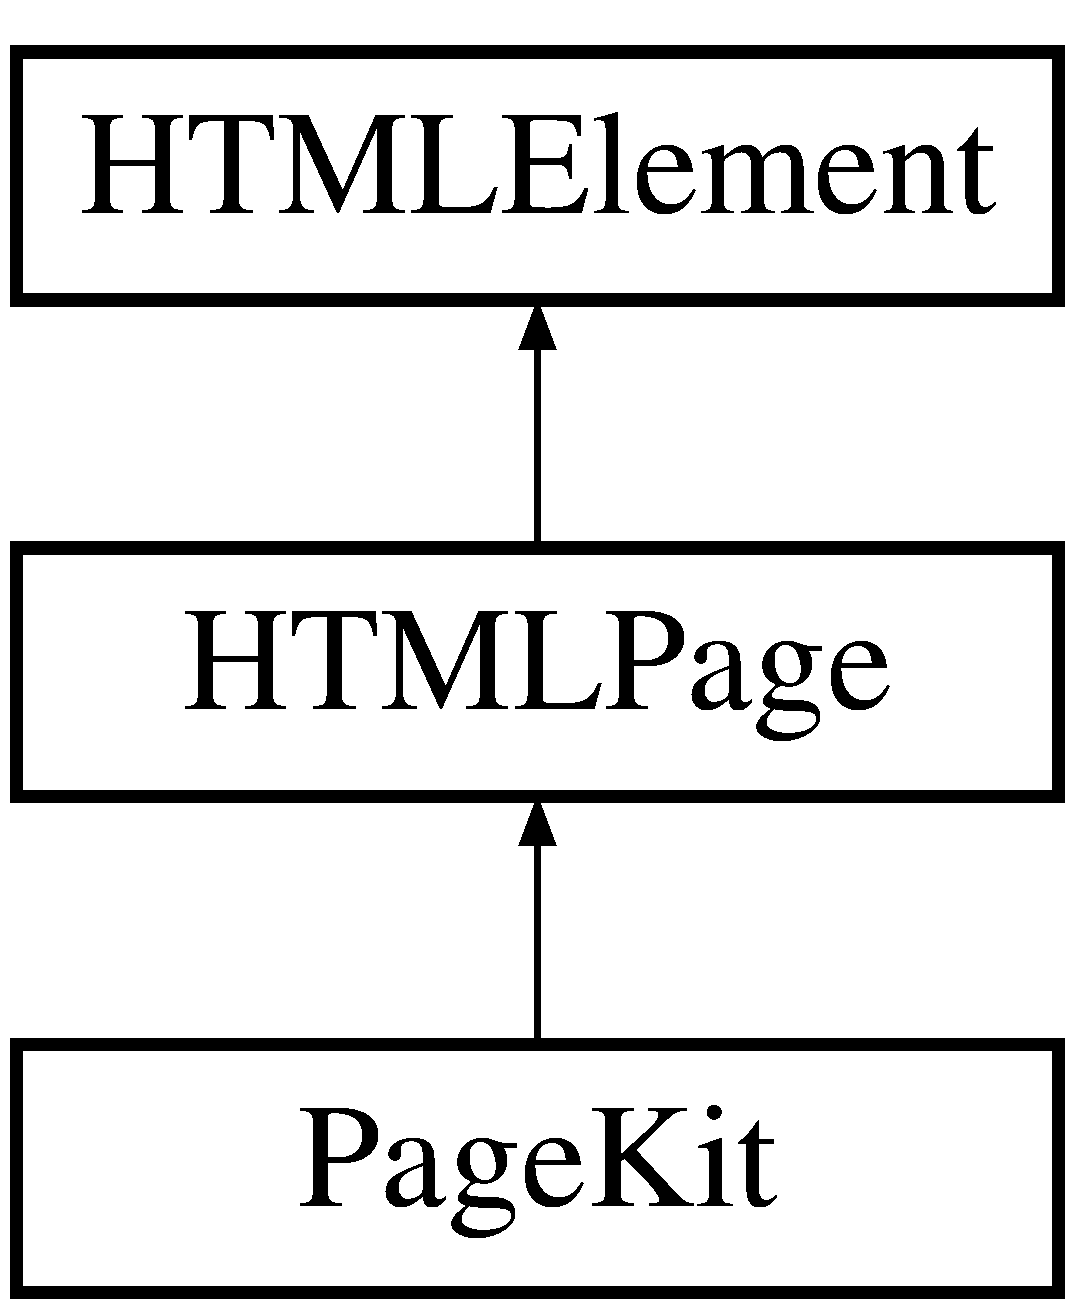
\includegraphics[height=3.000000cm]{class_page_kit}
\end{center}
\end{figure}
\subsection*{Public Member Functions}
\begin{DoxyCompactItemize}
\item 
\hyperlink{class_page_kit_a6220f56b893af1eeeaa7bb84f6ca13b2}{\-\_\-\-\_\-construct} (\$title)
\item 
\hyperlink{class_page_kit_a64e90a3db3b85412c4339f387e58e7a8}{Large\-Button} (\$url, \$text)
\item 
\hyperlink{class_page_kit_a6ee59b1624e21158bc52e1c7849bb3e9}{Medium\-Button} (\$url, \$text)
\item 
\hyperlink{class_page_kit_ae048b29e12fb2fe681c2c885cb2e32b8}{Small\-Button} (\$url, \$text)
\end{DoxyCompactItemize}
\subsection*{Additional Inherited Members}


\subsection{Constructor \& Destructor Documentation}
\hypertarget{class_page_kit_a6220f56b893af1eeeaa7bb84f6ca13b2}{\index{Page\-Kit@{Page\-Kit}!\-\_\-\-\_\-construct@{\-\_\-\-\_\-construct}}
\index{\-\_\-\-\_\-construct@{\-\_\-\-\_\-construct}!PageKit@{Page\-Kit}}
\subsubsection[{\-\_\-\-\_\-construct}]{\setlength{\rightskip}{0pt plus 5cm}\-\_\-\-\_\-construct (
\begin{DoxyParamCaption}
\item[{}]{\$title}
\end{DoxyParamCaption}
)}}\label{class_page_kit_a6220f56b893af1eeeaa7bb84f6ca13b2}


\subsection{Member Function Documentation}
\hypertarget{class_page_kit_a64e90a3db3b85412c4339f387e58e7a8}{\index{Page\-Kit@{Page\-Kit}!Large\-Button@{Large\-Button}}
\index{Large\-Button@{Large\-Button}!PageKit@{Page\-Kit}}
\subsubsection[{Large\-Button}]{\setlength{\rightskip}{0pt plus 5cm}Large\-Button (
\begin{DoxyParamCaption}
\item[{}]{\$url, }
\item[{}]{\$text}
\end{DoxyParamCaption}
)}}\label{class_page_kit_a64e90a3db3b85412c4339f387e58e7a8}
\hypertarget{class_page_kit_a6ee59b1624e21158bc52e1c7849bb3e9}{\index{Page\-Kit@{Page\-Kit}!Medium\-Button@{Medium\-Button}}
\index{Medium\-Button@{Medium\-Button}!PageKit@{Page\-Kit}}
\subsubsection[{Medium\-Button}]{\setlength{\rightskip}{0pt plus 5cm}Medium\-Button (
\begin{DoxyParamCaption}
\item[{}]{\$url, }
\item[{}]{\$text}
\end{DoxyParamCaption}
)}}\label{class_page_kit_a6ee59b1624e21158bc52e1c7849bb3e9}
\hypertarget{class_page_kit_ae048b29e12fb2fe681c2c885cb2e32b8}{\index{Page\-Kit@{Page\-Kit}!Small\-Button@{Small\-Button}}
\index{Small\-Button@{Small\-Button}!PageKit@{Page\-Kit}}
\subsubsection[{Small\-Button}]{\setlength{\rightskip}{0pt plus 5cm}Small\-Button (
\begin{DoxyParamCaption}
\item[{}]{\$url, }
\item[{}]{\$text}
\end{DoxyParamCaption}
)}}\label{class_page_kit_ae048b29e12fb2fe681c2c885cb2e32b8}


The documentation for this class was generated from the following file\-:\begin{DoxyCompactItemize}
\item 
\hyperlink{pagekit_8php}{pagekit.\-php}\end{DoxyCompactItemize}

\chapter{File Documentation}
\hypertarget{pagekit_8php}{\section{pagekit.\-php File Reference}
\label{pagekit_8php}\index{pagekit.\-php@{pagekit.\-php}}
}
\subsection*{Data Structures}
\begin{DoxyCompactItemize}
\item 
class \hyperlink{class_kit_settings}{Kit\-Settings}
\item 
class \hyperlink{class_color}{Color}
\item 
class \hyperlink{class_form}{Form}
\item 
class \hyperlink{class_listbox}{Listbox}
\item 
class \hyperlink{class_h_t_m_l_element}{H\-T\-M\-L\-Element}
\item 
class \hyperlink{class_h_t_m_l_page}{H\-T\-M\-L\-Page}
\item 
class \hyperlink{class_d_b_kit}{D\-B\-Kit}
\item 
class \hyperlink{class_file_kit}{File\-Kit}
\item 
class \hyperlink{class_page_kit}{Page\-Kit}
\item 
class \hyperlink{class_crypt_kit}{Crypt\-Kit}
\end{DoxyCompactItemize}
\subsection*{Functions}
\begin{DoxyCompactItemize}
\item 
\hyperlink{pagekit_8php_a16321ea290dabb36fceb18b44b356f81}{New\-Page} (\$title)
\item 
\hyperlink{pagekit_8php_abca823657bac21df9c14205c20cdd5bc}{New\-Form} (\$url)
\item 
\hyperlink{pagekit_8php_a859c2080642eca8f7b25efb5d8c4c523}{New\-Pagination} (\$previouslink, \$nextlink)
\item 
\hyperlink{pagekit_8php_a929d2a689ef203a7ef4f395fd29f53f2}{New\-Listbox} (\$id, \$name, \$size, \$multiple)
\item 
\hyperlink{pagekit_8php_a623ca09e2350244859902c7ced32a3b9}{New\-D\-B\-Connection} (\$settings)
\item 
\hyperlink{pagekit_8php_a8fc4d35b2a0ead87b02c2ac7a024a16a}{Settings} (\$dbhost, \$dbname, \$dbuser, \$dbpassword)
\end{DoxyCompactItemize}
\subsection*{Variables}
\begin{DoxyCompactItemize}
\item 
\hyperlink{pagekit_8php_ac7c3353107070daa85f641882931b358}{\$settings} = \hyperlink{pagekit_8php_a8fc4d35b2a0ead87b02c2ac7a024a16a}{Settings}(\char`\"{}localhost\char`\"{},\char`\"{}chonga\char`\"{},\char`\"{}root\char`\"{},\char`\"{}root\char`\"{})
\end{DoxyCompactItemize}


\subsection{Function Documentation}
\hypertarget{pagekit_8php_a623ca09e2350244859902c7ced32a3b9}{\index{pagekit.\-php@{pagekit.\-php}!New\-D\-B\-Connection@{New\-D\-B\-Connection}}
\index{New\-D\-B\-Connection@{New\-D\-B\-Connection}!pagekit.php@{pagekit.\-php}}
\subsubsection[{New\-D\-B\-Connection}]{\setlength{\rightskip}{0pt plus 5cm}New\-D\-B\-Connection (
\begin{DoxyParamCaption}
\item[{}]{\$settings}
\end{DoxyParamCaption}
)}}\label{pagekit_8php_a623ca09e2350244859902c7ced32a3b9}
New\-D\-B\-Connection(\$settings) This takes your settings and create and return a new database connection \hypertarget{pagekit_8php_abca823657bac21df9c14205c20cdd5bc}{\index{pagekit.\-php@{pagekit.\-php}!New\-Form@{New\-Form}}
\index{New\-Form@{New\-Form}!pagekit.php@{pagekit.\-php}}
\subsubsection[{New\-Form}]{\setlength{\rightskip}{0pt plus 5cm}New\-Form (
\begin{DoxyParamCaption}
\item[{}]{\$url}
\end{DoxyParamCaption}
)}}\label{pagekit_8php_abca823657bac21df9c14205c20cdd5bc}
New\-Form(\$url) This will create and return a new http form \hypertarget{pagekit_8php_a929d2a689ef203a7ef4f395fd29f53f2}{\index{pagekit.\-php@{pagekit.\-php}!New\-Listbox@{New\-Listbox}}
\index{New\-Listbox@{New\-Listbox}!pagekit.php@{pagekit.\-php}}
\subsubsection[{New\-Listbox}]{\setlength{\rightskip}{0pt plus 5cm}New\-Listbox (
\begin{DoxyParamCaption}
\item[{}]{\$id, }
\item[{}]{\$name, }
\item[{}]{\$size, }
\item[{}]{\$multiple}
\end{DoxyParamCaption}
)}}\label{pagekit_8php_a929d2a689ef203a7ef4f395fd29f53f2}
New\-Listbox(\$id,\$name, \$size,\$multiple) This will create and return a new http form List\-Box \hypertarget{pagekit_8php_a16321ea290dabb36fceb18b44b356f81}{\index{pagekit.\-php@{pagekit.\-php}!New\-Page@{New\-Page}}
\index{New\-Page@{New\-Page}!pagekit.php@{pagekit.\-php}}
\subsubsection[{New\-Page}]{\setlength{\rightskip}{0pt plus 5cm}New\-Page (
\begin{DoxyParamCaption}
\item[{}]{\$title}
\end{DoxyParamCaption}
)}}\label{pagekit_8php_a16321ea290dabb36fceb18b44b356f81}
New\-Page(\$title) This will create and return a new H\-T\-M\-L Page \hypertarget{pagekit_8php_a859c2080642eca8f7b25efb5d8c4c523}{\index{pagekit.\-php@{pagekit.\-php}!New\-Pagination@{New\-Pagination}}
\index{New\-Pagination@{New\-Pagination}!pagekit.php@{pagekit.\-php}}
\subsubsection[{New\-Pagination}]{\setlength{\rightskip}{0pt plus 5cm}New\-Pagination (
\begin{DoxyParamCaption}
\item[{}]{\$previouslink, }
\item[{}]{\$nextlink}
\end{DoxyParamCaption}
)}}\label{pagekit_8php_a859c2080642eca8f7b25efb5d8c4c523}
\hypertarget{pagekit_8php_a8fc4d35b2a0ead87b02c2ac7a024a16a}{\index{pagekit.\-php@{pagekit.\-php}!Settings@{Settings}}
\index{Settings@{Settings}!pagekit.php@{pagekit.\-php}}
\subsubsection[{Settings}]{\setlength{\rightskip}{0pt plus 5cm}Settings (
\begin{DoxyParamCaption}
\item[{}]{\$dbhost, }
\item[{}]{\$dbname, }
\item[{}]{\$dbuser, }
\item[{}]{\$dbpassword}
\end{DoxyParamCaption}
)}}\label{pagekit_8php_a8fc4d35b2a0ead87b02c2ac7a024a16a}
Settings This creates and returns database settings needed for D\-B Connection 

\subsection{Variable Documentation}
\hypertarget{pagekit_8php_ac7c3353107070daa85f641882931b358}{\index{pagekit.\-php@{pagekit.\-php}!\$settings@{\$settings}}
\index{\$settings@{\$settings}!pagekit.php@{pagekit.\-php}}
\subsubsection[{\$settings}]{\setlength{\rightskip}{0pt plus 5cm}\$settings = {\bf Settings}(\char`\"{}localhost\char`\"{},\char`\"{}chonga\char`\"{},\char`\"{}root\char`\"{},\char`\"{}root\char`\"{})}}\label{pagekit_8php_ac7c3353107070daa85f641882931b358}

%--- End generated contents ---

% Index
\newpage
\phantomsection
\addcontentsline{toc}{part}{Index}
\printindex

\end{document}
